\documentclass[oneside]{book}

% ------------------------------------------------------------------------------
% Packages
% ------------------------------------------------------------------------------

\usepackage[utf8]{inputenc}
\usepackage[english]{babel}

\usepackage{amsmath, amsthm, amssymb, amsfonts}
\usepackage{mathtools}

\usepackage[dvipsnames]{xcolor}
\usepackage{tcolorbox}
\tcbuselibrary{theorems, skins, breakable}

\usepackage{geometry}
\usepackage{setspace}
\usepackage{hyperref}
\usepackage{microtype}

\usepackage{multicol}
\setlength{\columnsep}{1.2em}

\usepackage{graphicx}

% ------------------------------------------------------------------------------
% Page Setup
% ------------------------------------------------------------------------------

\geometry{
    top=0.8in,
    bottom=0.8in,
    left=0.7in,
    right=0.7in,
    headheight=12pt,
    headsep=20pt,
    footskip=25pt
}

\setstretch{1.15}

\hypersetup{
    colorlinks=true,
    linkcolor=MidnightBlue,
    urlcolor=RoyalBlue,
    citecolor=ForestGreen
}

% ------------------------------------------------------------------------------
% Variables
% ------------------------------------------------------------------------------

\def\notetitle{Mathematics for the Slightly Rusty but Still Ambitious}
\def\notesubtitle{A Practical Review for Interviews, Work, and Future Moments of Panic}
\def\noteauthor{Erdan Mu Alan}
\def\noteinstitution{University of Pennsylvania}

% ------------------------------------------------------------------------------
% Theorem System and User Commands
% ------------------------------------------------------------------------------

% !TEX root = main.tex

% Theorem System
% The following boxes are provided:
%   Definition:     \defn 
%   Theorem:        \thm 
%   Lemma:          \lem
%   Corollary:      \cor
%   Proposition:    \prop   
%   Claim:          \clm
%   Fact:           \fact
%   Proof:          \pf
%   Example:        \ex
%   Remark:         \rmk (sentence), \rmkb (block)
% Suffix
%   r:              Allow Theorem/Definition to be referenced, e.g. thmr
%   p:              Add a short proof block for Lemma, Corollary, Proposition or Claim, e.g. lemp
%                   For theorems, use \pf for proof blocks

\tcbset{
    kb/common block/.style={
        enhanced,
        breakable,
        frame hidden,
        boxrule=0pt,
        sharp corners,
        boxsep=0pt,
        left=6mm,
        right=5mm,
        top=4mm,
        bottom=4mm,
        before skip=10pt,
        after skip=12pt,
        before upper={\parindent15pt\relax},
    },
    kb/proof block/.style={
        kb/common block,
        colback=black!1!white,
        borderline west={0.9mm}{0pt}{black!55},
    },
    kb/accent proof/.style n args={2}{
        kb/common block,
        colback=#1!4!white,
        borderline west={1mm}{0pt}{#1},
        before upper={
            \parindent15pt\relax
            {\noindent\bfseries #2}\par\smallskip
        },
    },
    kb/example block/.style={
        kb/common block,
        colback=MidnightBlue!3!white,
        borderline west={1.2mm}{0pt}{MidnightBlue!70!black},
        borderline north={0.3mm}{0pt}{MidnightBlue!18!white},
    },
    kb/example title/.style={
        colback=MidnightBlue!75!black,
        colframe=MidnightBlue!75!black,
        boxrule=0pt,
        sharp corners,
        left=3mm,
        right=3mm,
        top=1.2mm,
        bottom=1.2mm,
    },
}

\newcounter{example}[section]
\renewcommand{\theexample}{\thesection.\arabic{example}}

% Definition
\newtcbtheorem[number within=section]{mydefinition}{Definition}
{
    enhanced,
    frame hidden,
    titlerule=0mm,
    toptitle=1mm,
    bottomtitle=1mm,
    fonttitle=\bfseries\large,
    coltitle=black,
    colbacktitle=blue!20!white,
    colback=blue!10!white,
}{defn}

\NewDocumentCommand{\defn}{m+m}{
    \begin{mydefinition}{#1}{}
        #2
    \end{mydefinition}
}

\NewDocumentCommand{\defnr}{mm+m}{
    \begin{mydefinition}{#1}{#2}
        #3
    \end{mydefinition}
}

\NewDocumentEnvironment{definition}{o+b}{
    \IfNoValueTF{#1}{
        \begin{mydefinition}{}{}
    }{
        \begin{mydefinition}{#1}{}
    }
    #2
    \end{mydefinition}
}{}

% Theorem
\newtcbtheorem[use counter from=mydefinition]{mytheorem}{Theorem}
{
    enhanced,
    frame hidden,
    titlerule=0mm,
    toptitle=1mm,
    bottomtitle=1mm,
    fonttitle=\bfseries\large,
    coltitle=black,
    colbacktitle=cyan!20!white,
    colback=cyan!10!white,
}{thm}

\NewDocumentCommand{\thm}{m+m}{
    \begin{mytheorem}{#1}{}
        #2
    \end{mytheorem}
}

\NewDocumentCommand{\thmr}{mm+m}{
    \begin{mytheorem}{#1}{#2}
        #3
    \end{mytheorem}
}

\NewDocumentEnvironment{theorem}{o+b}{
    \IfNoValueTF{#1}{
        \begin{mytheorem}{}{}
    }{
        \begin{mytheorem}{#1}{}
    }
    #2
    \end{mytheorem}
}{}

% Lemma
\newtcbtheorem[use counter from=mydefinition]{mylemma}{Lemma}
{
    enhanced,
    frame hidden,
    titlerule=0mm,
    toptitle=1mm,
    bottomtitle=1mm,
    fonttitle=\bfseries\large,
    coltitle=black,
    colbacktitle=violet!20!white,
    colback=violet!10!white,
}{lem}

\NewDocumentCommand{\lem}{m+m}{
    \begin{mylemma}{#1}{}
        #2
    \end{mylemma}
}

\newenvironment{lempf}{
    \begin{tcolorbox}[kb/accent proof={violet!65!black}{Proof for Lemma.}]
}{
    \hfill\textcolor{violet!65!black}{$\blacksquare$}
    \end{tcolorbox}
}

\NewDocumentCommand{\lemp}{m+m+m}{
    \begin{mylemma}{#1}{}
        #2
    \end{mylemma}

    \begin{lempf}
        #3
    \end{lempf}
}

% Corollary
\newtcbtheorem[use counter from=mydefinition]{mycorollary}{Corollary}
{
    enhanced,
    frame hidden,
    titlerule=0mm,
    toptitle=1mm,
    bottomtitle=1mm,
    fonttitle=\bfseries\large,
    coltitle=black,
    colbacktitle=orange!20!white,
    colback=orange!10!white,
}{cor}

\NewDocumentCommand{\cor}{+m}{
    \begin{mycorollary}{}{}
        #1
    \end{mycorollary}
}

\newenvironment{corpf}{
    \begin{tcolorbox}[kb/accent proof={orange!80!black}{Proof for Corollary.}]
}{
    \hfill\textcolor{orange!80!black}{$\blacksquare$}
    \end{tcolorbox}
}

\NewDocumentCommand{\corp}{m+m+m}{
    \begin{mycorollary}{}{}
        #1
    \end{mycorollary}

    \begin{corpf}
        #2
    \end{corpf}
}

% Proposition
\newtcbtheorem[use counter from=mydefinition]{myproposition}{Proposition}
{
    enhanced,
    frame hidden,
    titlerule=0mm,
    toptitle=1mm,
    bottomtitle=1mm,
    fonttitle=\bfseries\large,
    coltitle=black,
    colbacktitle=yellow!30!white,
    colback=yellow!20!white,
}{prop}

\NewDocumentCommand{\prop}{+m}{
    \begin{myproposition}{}{}
        #1
    \end{myproposition}
}

\newenvironment{proppf}{
    \begin{tcolorbox}[kb/accent proof={Goldenrod!85!black}{Proof for Proposition.}]
}{
    \hfill\textcolor{Goldenrod!85!black}{$\blacksquare$}
    \end{tcolorbox}
}

\NewDocumentCommand{\propp}{+m+m}{
    \begin{myproposition}{}{}
        #1
    \end{myproposition}

    \begin{proppf}
        #2
    \end{proppf}
}

% Claim
\newtcbtheorem[use counter from=mydefinition]{myclaim}{Claim}
{
    enhanced,
    frame hidden,
    titlerule=0mm,
    toptitle=1mm,
    bottomtitle=1mm,
    fonttitle=\bfseries\large,
    coltitle=black,
    colbacktitle=pink!30!white,
    colback=pink!20!white,
}{clm}


\NewDocumentCommand{\clm}{m+m}{
    \begin{myclaim*}{#1}{}
        #2
    \end{myclaim*}
}

\newenvironment{clmpf}{
    \begin{tcolorbox}[kb/accent proof={Magenta!70!black}{Proof for Claim.}]
}{
    \hfill\textcolor{Magenta!70!black}{$\blacksquare$}
    \end{tcolorbox}
}

\NewDocumentCommand{\clmp}{m+m+m}{
    \begin{myclaim*}{#1}{}
        #2
    \end{myclaim*}

    \begin{clmpf}
        #3
    \end{clmpf}
}

% Fact
\newtcbtheorem[use counter from=mydefinition]{myfact}{Fact}
{
    enhanced,
    frame hidden,
    titlerule=0mm,
    toptitle=1mm,
    bottomtitle=1mm,
    fonttitle=\bfseries\large,
    coltitle=black,
    colbacktitle=purple!20!white,
    colback=purple!10!white,
}{fact}

\NewDocumentCommand{\fact}{+m}{
    \begin{myfact}{}{}
        #1
    \end{myfact}
}


% Proof
\RenewDocumentEnvironment{proof}{O{\proofname}}{
    \par
    \pushQED{\qed}
    \begin{tcolorbox}[kb/proof block]
        {\noindent\bfseries #1}\par\smallskip
        \ignorespaces
}{
    \popQED
    \end{tcolorbox}
    \par
}

\let\proofenvironment\proof
\let\endproofenvironment\endproof

\makeatletter
\renewcommand{\proof}{
    \@ifnextchar\bgroup{\proofcommand}{\proofenvironment}
}
\makeatother

\NewDocumentCommand{\proofcommand}{+m}{
    \proofenvironment
        #1
    \endproofenvironment
}

\NewDocumentCommand{\pf}{o+m}{
    \IfNoValueTF{#1}{
        \begin{proof}
            #2
        \end{proof}
    }{
        \begin{proof}[#1]
            #2
        \end{proof}
    }
}

% Example
\NewDocumentEnvironment{example}{o+b}{
    \refstepcounter{example}
    \IfNoValueTF{#1}{
        \def\exampletitle{Example \theexample}
    }{
        \def\exampletitle{Example \theexample \textbar\ #1}
    }
    \begin{tcolorbox}[
        kb/example block,
        title={\exampletitle},
        fonttitle=\bfseries\small,
        coltitle=white,
        boxed title style={kb/example title},
        attach boxed title to top left={xshift=4mm,yshift*=-\tcboxedtitleheight/2},
        top=7mm,
    ]
        #2
    \end{tcolorbox}
}{}

\NewDocumentCommand{\ex}{+m}{
    \begin{example}
        #1
    \end{example}
}


% Remark
\NewDocumentCommand{\rmk}{+m}{
    {\it \color{blue!50!white}#1}
}

\newenvironment{remark}{
    \par
    \vspace{5pt}
    \begin{minipage}{\textwidth}
        {\par\noindent{\textbf{Remark.}}}
        \tcolorbox[blanker,breakable,left=5mm,
        before skip=10pt,after skip=10pt,
        borderline west={1mm}{0pt}{cyan!10!white}]
}{
        \endtcolorbox
    \end{minipage}
    \vspace{5pt}
}

\NewDocumentCommand{\rmkb}{+m}{
    \begin{remark}
        #1
    \end{remark}
}

% !TEX root = main.tex

\newcommand{\R}{\mathbb{R}}
\newcommand{\N}{\mathbb{N}}
\newcommand{\vect}[1]{\mathbf{#1}}
\newcommand{\norm}[1]{\left\lVert #1 \right\rVert}
\newcommand{\dd}{\mathop{}\!\mathrm{d}}
\newcommand{\grad}{\nabla}
\newcommand{\diver}{\operatorname{div}}
\newcommand{\pd}[2]{\frac{\partial #1}{\partial #2}}
\newcommand{\lcm}{\operatorname{lcm}}


% ------------------------------------------------------------------------------
% Document
% ------------------------------------------------------------------------------

\begin{document}

% ------------------------------------------------------------------------------
% Title Page
% ------------------------------------------------------------------------------

\begin{titlepage}
    \centering

    \vspace*{2.2cm}

    {\Huge\bfseries \notetitle \par}

    \vspace{0.9cm}

    \resizebox{0.88\textwidth}{!}{%
        \itshape \notesubtitle
    }

    \vspace{2.4cm}

    \vspace{1.2cm}

    {\large \noteauthor \par}

    \vspace{0.25cm}

    {\large \noteinstitution \par}

    \vfill
\end{titlepage}

% ------------------------------------------------------------------------------
% Front Matter
% ------------------------------------------------------------------------------

\frontmatter
\setcounter{tocdepth}{1}
\tableofcontents
\newpage

% ------------------------------------------------------------------------------
% Main Matter
% ------------------------------------------------------------------------------

\mainmatter


\chapter{Multivariable Calculus}

\section{Limits, Continuity, and Derivatives}

\defn{Function}{
    A \emph{function} $f:D\to E$ is a rule that assigns to each element $x\in D$ exactly one element $f(x)\in E$. The set $D$ is the \emph{domain}, and the set of all actual output values is the \emph{range}.
}
\paragraph{Increasing and Decreasing Functions}{
    Let $f$ be defined on an interval $I$: 
    \begin{itemize}
        \item Whenever $x_1<x_2$ in $I$, $f$ is \emph{increasing} on $I$ if $f(x_1)<f(x_2)$, is \emph{nondecreasing} on $I$ if $f(x_1)\le f(x_2)$.
        \item Whenever $x_1<x_2$ in $I$, $f$ is \emph{decreasing} on $I$ if $f(x_1)>f(x_2)$, is \emph{nonincreasing} on $I$ if $f(x_1)\ge f(x_2)$.
    \end{itemize}
}

\paragraph{Informal Definition of Limit} The statement $\lim_{x\to a} f(x)=L$ means that $f(x)$ can be made arbitrarily close to $L$ by taking $x$ sufficiently close to $a$, from both the left and the right, but with $x\ne a$.

\paragraph{Right- and Left-Hand Limits}{
    $\lim_{x\to a^+} f(x)=L$ means that $f(x)$ can be made arbitrarily close to $L$ by taking $x$ sufficiently close to $a$ with $x>a$. Similarly. $\lim_{x\to a^-} f(x)=L$ means that $x$ approaches $a$ from the left, so $x<a$.
}

\paragraph{Two-Sided Limit}{
    The two-sided limit exists and equals $L$ if and only if:
    \[
        \lim_{x\to a} f(x)=L
        \quad\Longleftrightarrow\quad
        \lim_{x\to a^-} f(x)=L
        \text{ and }
        \lim_{x\to a^+} f(x)=L
    \]
}

\paragraph{Vertical Asymptote}{
    The line $x=a$ is a \emph{vertical asymptote} of the graph of $f$ if at least one of the following is true:
    \[
        \lim_{x\to a^-}f(x)=\pm\infty,
        \qquad
        \lim_{x\to a^+}f(x)=\pm\infty
    \]
}

\thmr{Squeeze Theorem}{squeezetheorem}{
    Suppose $g(x)\le f(x)\le h(x)$ for all $x$ near $a$. If $\lim_{x\to a}g(x)=L$ and $\lim_{x\to a}h(x)=L$, then $\lim_{x\to a}f(x)=L$.
}

\defn{Formal Definition of Limit}{
    Let $f$ be defined near $a$, except possibly at $a$. We say $\lim_{x\to a}f(x)=L$ if for every $\varepsilon>0$, there exists $\delta>0$ such that whenever $0<|x-a|<\delta$, 
    we have $|f(x)-L|<\varepsilon$. 
}

\ex{
    \noindent Proof that $\lim_{x\to 2}\frac{x^2-4}{x-2}=4$. Let $\varepsilon>0$ be given. Choose $\delta=\varepsilon$. If
    $0<|x-2|<\delta$, then $x\neq 2$, so $\left|\frac{x^2-4}{x-2}-4\right|=\left|\frac{(x-2)(x+2)}{x-2}-4\right|=|x+2-4|=|x-2|<\delta=\varepsilon$. 
    Thus, by the $\varepsilon$-$\delta$ definition, $\lim_{x\to 2}\frac{x^2-4}{x-2}=4$. 
}

\paragraph{Continuity at a Point}{
    A function $f:D\to \mathbb{R}$ is \emph{continuous at} $a\in D$ if $\lim_{x\to a}f(x)=f(a)$. 
}

\paragraph{Continuity on an Interval}{
    A function is \emph{continuous on an interval} if it is continuous at every point of that interval. At endpoints, continuity is understood using the appropriate one-sided limit.
}

\paragraph{Types of Discontinuity.}
Typical discontinuities include:
\begin{itemize}
    \item \emph{removable discontinuity}: the limit exists but $f(a)$ is missing or has the wrong value;
    \item \emph{jump discontinuity}: the one-sided limits exist but are not equal;
    \item \emph{infinite discontinuity}: the function tends to $\pm\infty$;
    \item \emph{oscillatory discontinuity}: the function oscillates and has no limiting value.
\end{itemize}

\thmr{Intermediate Value Theorem}{ivt}{
    Suppose $f$ is continuous on the closed interval $[a,b]$. If $N$ is any number between $f(a)$ and $f(b)$, then there exists at least one $c\in[a,b]$ such that $f(c)=N$. 
}

\paragraph{Limit at Infinity}{
    $\lim_{x\to +\infty}f(x)=L$ means that $\forall \varepsilon>0$, there exists $N>0$ such that if $x>N$, then $|f(x)-L|<\varepsilon$. Similarily,
    $ \lim_{x\to -\infty}f(x)=L$ means that $\forall \varepsilon>0$, there exists $N>0$ such that if $x<-N$, then $|f(x)-L|<\varepsilon$. 
}

\paragraph{Horizontal Asymptote}{
    The line $y=L$ is a \emph{horizontal asymptote} if
    \[
        \lim_{x\to +\infty}f(x)=L
        \quad\text{or}\quad
        \lim_{x\to -\infty}f(x)=L
    \]
}

\paragraph{Tangent Line}{
    If the limit $m=\lim_{x\to a}\frac{f(x)-f(a)}{x-a}$
    exists, then the tangent line to the graph of $f$ at $(a,f(a))$ is
    \[
        y-f(a)=m(x-a)
    \]
}

\defn{Derivative at a Point}{
    The derivative of $f$ at $a$ is
    \[
        f'(a)=\lim_{x\to a}\frac{f(x)-f(a)}{x-a}=\lim_{h\to 0}\frac{f(a+h)-f(a)}{h}
    \]
}

\rmk{
    The derivative is the slope of the tangent line and the instantaneous rate of change of $f$ at $a$.
}

\paragraph{Derivative Function}{
    The derivative of $f$ is the function defined at all $x$ where this limit exists: 
    \[
        f'(x)=\lim_{h\to 0}\frac{f(x+h)-f(x)}{h}
    \]
}

\paragraph{Differentiability Implies Continuity}{diffimpliescont}{
    If $f$ is differentiable at $a$, then $f$ is continuous at $a$.
}

\rmk{
    The converse is false. A function can be continuous but not differentiable. $f(x) = |x|$. 
}

\paragraph{Basic Differentiation Rules}{
    Let $c\in\mathbb{R}$ and suppose $f,g$ are differentiable. Then
    \begin{align*}
        \frac{d}{dx}[c] =0 \qquad 
        \frac{d}{dx}[x^n] = nx^{n-1} \qquad
        \frac{d}{dx}[cf(x)] = c f'(x) \qquad
        \frac{d}{dx}[f(x) \pm g(x)] &= f'(x) \pm g'(x)
    \end{align*}
}

\paragraph{Product Rule and Quotient Rule}{productrule}{
    If $f$ and $g$ are differentiable, then $fg$ is differentiable and
    \[
        \frac{d}{dx}[f(x)g(x)]
        =f'(x)g(x)+f(x)g'(x) \qquad
        \frac{d}{dx}\left[\frac{f(x)}{g(x)}\right]
        =\frac{f'(x)g(x)-f(x)g'(x)}{[g(x)]^2}
    \]
}

\paragraph{Derivative Formulas for Trigonometric Functions}{
    \[
        \frac{d}{dx}\sin x = \cos x \qquad
        \frac{d}{dx}\cos x = -\sin x \qquad
        \frac{d}{dx}\tan x = \sec^2 x 
    \]
    \[
        \frac{d}{dx}\cot x = -\csc^2 x \qquad
        \frac{d}{dx}\sec x = \sec x\tan x \qquad
        \frac{d}{dx}\csc x = -\csc x\cot x 
    \]
}

\thmr{Chain Rule}{chainrule}{
    If $g$ is differentiable at $x$ and $f$ is differentiable at $g(x)$, let $y=f(u)$ and $u=g(x)$, then
    \[
        \frac{d}{dx}f(g(x))=f'(g(x))g'(x) \qquad \frac{dy}{dx}=\frac{dy}{du}\frac{du}{dx}
    \]
}

\begin{proof}
\noindent Assume first that \(g(x)\neq g(a)\) for \(x\) sufficiently close to \(a\), \(x\neq a\). Then
\[
(f\circ g)'(a)
=\lim_{x \rightarrow a}\frac{f(g(x))-f(g(a))}{x-a}
=\lim_{x \rightarrow a}\frac{f(g(x))-f(g(a))}{g(x)-g(a)} \cdot \frac{g(x)-g(a)}{x-a}
=f'(g(a))g'(a)
\]
\end{proof}

\paragraph{Inverse Function Derivative}{inversefunctionderivative}{
    \[
        (f^{-1})'(x)=\frac{1}{f'(f^{-1}(x))}
    \]
}

\paragraph{Exponential and Logarithm Derivatives}{
    \[
        \frac{d}{dx}e^x=e^x \qquad \frac{d}{dx}a^x=a^x\ln a
    \]
    \[
        \frac{d}{dx}\ln x=\frac{1}{x} \qquad \frac{d}{dx} \log_a x = \frac{1}{x \ln a}
    \]
}

\paragraph{Inverse Trigonometric Derivatives}{
    \begin{align*}
        \frac{d}{dx}\arcsin x = \frac{1}{\sqrt{1-x^2}} \qquad
        \frac{d}{dx}\arccos x = -\frac{1}{\sqrt{1-x^2}} \qquad
        \frac{d}{dx}\arctan x = \frac{1}{1+x^2} 
    \end{align*}
}

\paragraph{Implicit Derivative}{
    A function may be defined implicitly by a relation between $x$ and $y$; instead of solving for $y$ explicitly, differentiate both sides with respect to $x$, treating $y$ as a function of $x$, and apply the chain rule when differentiating expressions involving $y$, e.g. $\dfrac{d}{dx}[y]=y'$, $\dfrac{d}{dx}[y^2]=2yy'$, $\dfrac{d}{dx}[\sin y]=\cos(y)y'$.    
}

\paragraph{Linearization}{
If $f$ is differentiable at $x=a$, the \textbf{linearization} of $f$ at $a$ is
$L(x)=f(a)+f'(a)(x-a)$.
}

\paragraph{Differential}{
If $y=f(x)$, then $dy=f'(x)\,dx$. The actual change is
$\Delta y=f(x+\Delta x)-f(x) \approx dy=f'(x)\Delta x, \Delta x \rightarrow 0$. 
}

\thm{Extreme Value Theorem}{
If $f$ is continuous on a closed interval $[a,b]$, then $f$ attains both an absolute maximum and minimum on $[a,b]$.
}

\paragraph{Local and Absolute Extremum}{
    \begin{itemize}
        \item $f$ has a \textbf{local maximum} at $c$ if $f(c)\ge f(x)$ for all $x$ sufficiently close to $c$. 
        \item $f$ has a \textbf{local minimum} at $c$ if $f(c)\le f(x)$ for all $x$ sufficiently close to $c$. 
        \item $f$ has an \textbf{absolute maximum} at $c$ on a domain $D$ if $f(c)\ge f(x)\qquad \text{for all }x\in D$.
        \item $f$ has an \textbf{absolute minimum} at $c$ on a domain $D$ if $f(c)\le f(x)\qquad \text{for all }x\in D$. 
    \end{itemize}
}

\paragraph{Critical Number}{
A number $c$ in the domain of $f$ is a \textbf{critical number} if $f'(c)=0$ or $f'(c)\text{ does not exist}$. 
}

\paragraph{Closed Interval Method}{
To find absolute extrema of a continuous function $f$ on $[a,b]$:
\begin{enumerate}
    \item Find all critical numbers in $(a,b)$.
    \item Evaluate $f$ at the critical numbers. Evaluate $f(a)$ and $f(b)$. Compare all values.
\end{enumerate}
}

\thm{Rolle's Theorem}{
Suppose $f$ is continuous on $[a,b]$, $f$ is differentiable on $(a,b)$, and $f(a)=f(b)$, then $\exists c\in(a,b)$ such that 
    \[f'(c)=0\]
}

\begin{proof}
\noindent Since \(f\) is continuous on \([a,b]\), by the Extreme Value Theorem,
\(f\) attains a maximum and a minimum on \([a,b]\). If \(f\) is constant on \([a,b]\), then \(f'(x)=0\) for every
\(x\in(a,b)\), so the result holds. Assume \(f\) is not constant. Since \(f(a)=f(b)\), at least one of the
maximum or minimum values of \(f\) is attained at some interior point
\(c\in(a,b)\). Thus \(f\) has a local maximum or local minimum at \(c\). Because \(f\) is differentiable on \((a,b)\), Fermat's Theorem gives
$
f'(c)=0.
$
Therefore, there exists \(c\in(a,b)\) such that
$
f'(c)=0.
$
\end{proof}

\thm{Mean Value Theorem}{
Suppose $f$ is continuous on $[a,b]$ and $f$ is differentiable on $(a,b)$ then there exists $c\in(a,b)$ such that
\[
f'(c)=\frac{f(b)-f(a)}{b-a}
\]
}

\begin{proof}
Let
$
m=\frac{f(b)-f(a)}{b-a}.
$
Consider the secant line
$
L(x)=f(a)+m(x-a),
$
and define
$
g(x)=f(x)-L(x).
$
Since \(f\) is continuous on \([a,b]\) and differentiable on \((a,b)\), and \(L\) is linear, \(g\) is also continuous on \([a,b]\) and differentiable on \((a,b)\). Moreover,
$
g(a)=f(a)-L(a)=f(a)-f(a)=0,
$
and
$
g(b)=f(b)-L(b)
=f(b)-\left(f(a)+m(b-a)\right)
=f(b)-\left(f(a)+f(b)-f(a)\right)=0.
$
Thus \(g(a)=g(b)\). By Rolle's Theorem, there exists \(c\in(a,b)\) such that
$
g'(c)=0.
$
But
$
g'(x)=f'(x)-L'(x)=f'(x)-m.
$
Therefore,
$
f'(c)=m=\frac{f(b)-f(a)}{b-a}.
$
\end{proof}

\paragraph{First Derivative Test}{
Let $c$ be a critical number: 
\begin{enumerate}
    \item If $f'$ changes from positive to negative at $c$, then $f$ has a local maximum at $c$.
    \item If $f'$ changes from negative to positive at $c$, then $f$ has a local minimum at $c$.
    \item If $f'$ does not change sign at $c$, then $f$ has no local extremum at $c$.
\end{enumerate}
}

\paragraph{Concavity}{
    \begin{enumerate}
        \item $f$ is \textbf{concave up} on an interval if $f''(x)>0$ on that interval.
        \item $f$ is \textbf{concave down} on an interval if $f''(x)<0$ on that interval.
    \end{enumerate}
}

\paragraph{Second Derivative Test}{
Suppose $f'(c)=0$: 
\begin{enumerate}
    \item If $f''(c)>0$, then $f$ has a local minimum at $c$.
    \item If $f''(c)<0$, then $f$ has a local maximum at $c$.
    \item If $f''(c)=0$, the test is inconclusive.
\end{enumerate}
}

\paragraph{Inflection Point}{
A point $x=c$ is an \textbf{inflection point} if $f$ is continuous at $c$ and concavity changes at $c$. Possible candidates occur when
$f''(c)=0$ or $f''(c)\text{ does not exist}$
}

\thm{L'Hopital's Rule}{
If $\lim_{x\to a}f(x)=\lim_{x\to a}g(x)=0$ or both limits are infinite, and if
$\lim_{x\to a}\frac{f'(x)}{g'(x)}$ exists or equals $\pm\infty$, then
\[
\lim_{x\to a}\frac{f(x)}{g(x)}=\lim_{x\to a}\frac{f'(x)}{g'(x)}
\]
}

\section{Integrations and the Fundamental Theorem of Calculus}

\paragraph{Area Approximation}{
On $[a,b]$, $\Delta x=\frac{b-a}{n}$.
Right endpoint: $x_i=a+i\Delta x$. 
Left endpoint: $x_{i-1}=a+(i-1)\Delta x$.
Midpoint: $\bar{x}_i=a+\left(i-\frac12\right)\Delta x$.
The approximate area is $\sum_{i=1}^n f(x_i^*)\Delta x$.
}

\defn{Definite Integral}{
If the limit exists, let $\Delta x=\frac{b-a}{n}$: 
\[
\int_a^b f(x)\,dx=\lim_{n\to\infty}\sum_{i=1}^n f(x_i^*)\Delta x
\]
}

\rmk{
A definite integral is signed area. Area above the $x$-axis is positive; area below is negative.
}

\paragraph{Properties}
\[
\int_a^a f(x)\,dx=0
\qquad
\int_a^b f(x)\,dx=-\int_b^a f(x)\,dx
\qquad
\int_a^b cf(x)\,dx=c\int_a^b f(x)\,dx
\]
\[
\int_a^b [f(x)+g(x)]\,dx=\int_a^b f(x)\,dx+\int_a^b g(x)\,dx
\qquad
\int_a^b f(x)\,dx=\int_a^c f(x)\,dx+\int_c^b f(x)\,dx
\]

\paragraph{Antiderivative}{
$F$ is an antiderivative of $f$ if $F'(x)=f(x)$. All antiderivatives are $F(x)+C$. 
}

\thm{Fundamental Theorem of Calculus Part 1}{
    If $f$ is continuous and $g(x)=\int_a^x f(t)\,dt$ then $g'(x)=f(x)$.
}

\begin{center}
\IfFileExists{math_imgs/FTC_1.png}{
    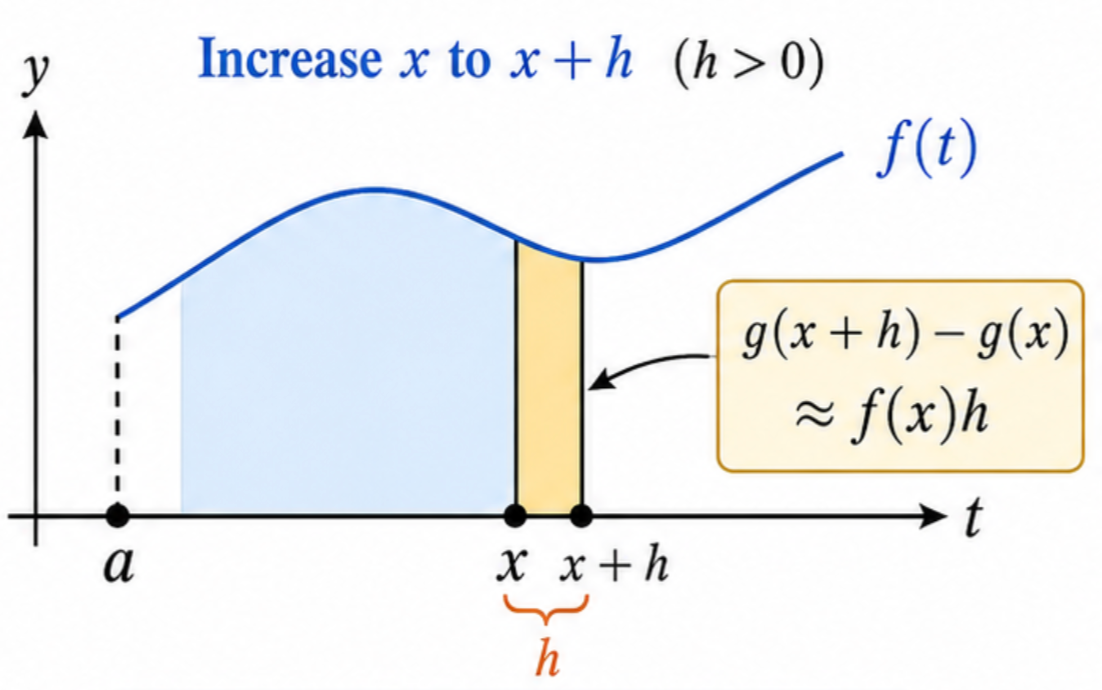
\includegraphics[width=0.4\textwidth]{math_imgs/FTC_1.png}
}{
    \fbox{
        \parbox[c][0.15\textheight][c]{0.4\textwidth}{
            \centering
            Add \texttt{math\_imgs/FTC\_1.png}
        }
    }
}
\end{center}

\rmk{The rate of change of accumulated area is the current height of the function.}

\begin{proof}
\noindent By the definition of derivative,
$
    g'(x)=\lim_{h\to 0}\frac{g(x+h)-g(x)}{h}.
$
Since
$
    g(x+h)-g(x)
    =
    \int_a^{x+h}f(t)\,dt-\int_a^x f(t)\,dt
    =
    \int_x^{x+h}f(t)\,dt,
$
we have
$
    g'(x)
    =
    \lim_{h\to 0}\frac{1}{h}\int_x^{x+h}f(t)\,dt.
$
Because \(f\) is continuous, the average value of \(f\) on \([x,x+h]\)
approaches \(f(x)\) as \(h\to 0\). Hence
$
    \lim_{h\to 0}\frac{1}{h}\int_x^{x+h}f(t)\,dt
    =
    f(x).
$
Therefore, \(g'(x)=f(x)\).
\end{proof}

\thm{Fundamental Theorem of Calculus Part 2}{
If $f$ is continuous on $[a,b]$ and $F'(x)=f(x)$, then
\[
\int_a^b f(x)\,dx=F(b)-F(a)
\]
}

\rmk{Adding up infinitely many tiny changes $f(x)dx$ gives the total change $F(b)-F(a)$ from $a$ to $b$.}

\begin{proof}
\noindent Define
$
    g(x)=\int_a^x f(t)\,dt.
$
By the Fundamental Theorem of Calculus Part 1,
$
    g'(x)=f(x).
$
Since \(F'(x)=f(x)\), we have
$
    g'(x)=F'(x).
$
Therefore, for some constant \(C\),
$
    g(x)=F(x)+C.
$
Evaluating at \(x=a\), we get
$
    g(a)=\int_a^a f(t)\,dt=0.
$
Hence
$
    C=-F(a).
$
Therefore,
$
    g(x)=F(x)-F(a).
$
Setting \(x=b\), we obtain the result. 
\end{proof}

\paragraph{Substitution Rule}
If $u=g(x), du=g'(x)\,dx$, then 
\[
\int f(g(x))g'(x)\,dx=\int f(u)\,du
\]
For definite integrals, change the bounds:
\[
\int_a^b f(g(x))g'(x)\,dx=\int_{g(a)}^{g(b)} f(u)\,du
\]

\paragraph{Integration by Parts}{
\[
\int u\,dv=uv-\int v\,du
\]
For definite integrals,
\[
\int_a^b u\,dv=[uv]_a^b-\int_a^b v\,du
\]
}

\paragraph{Partial Fractions}
For a proper rational function $P(x)/Q(x)$ (where $\deg P<\deg Q$):
\begin{itemize}
\item \textbf{Distinct linear:} $(x-a)(x-b) \to \frac{A}{x-a}+\frac{B}{x-b}$
\item \textbf{Repeated linear:} $(x-a)^r \to \frac{A_1}{x-a}+\cdots+\frac{A_r}{(x-a)^r}$
\item \textbf{Irreducible quadratic:} $ax^2+bx+c \to \frac{Ax+B}{ax^2+bx+c}$
\end{itemize}
Key integrals:
\[
\int \frac{dx}{ax+b}=\frac1a\ln|ax+b|+C, \quad \int \frac{dx}{x^2+a^2}=\frac1a\arctan\left(\frac xa\right)+C
\]

\paragraph{Infinite Intervals}
\[
\int_a^\infty f(x)\,dx=\lim_{t\to\infty}\int_a^t f(x)\,dx
\]
\[
\int_{-\infty}^b f(x)\,dx=\lim_{t\to-\infty}\int_t^b f(x)\,dx
\]
For $\int_{-\infty}^{\infty} f(x)\,dx$ split at any $c$:
\[
\int_{-\infty}^{\infty} f(x)\,dx=\int_{-\infty}^{c} f(x)\,dx+\int_c^\infty f(x)\,dx.
\]

\paragraph{Comparison Theorem}{
If $0\le f(x)\le g(x)$ on $[a,\infty)$, then:
\begin{enumerate}
    \item If $\int_a^\infty g(x)\,dx$ converges, then $\int_a^\infty f(x)\,dx$ converges.
    \item If $\int_a^\infty f(x)\,dx$ diverges, then $\int_a^\infty g(x)\,dx$ diverges.
\end{enumerate}
}

\paragraph{Absolute Area}
If $f$ crosses the $x$-axis, geometric area is below, split at zeros of $f$ and remove negative signed area:
\[
A=\int_a^b |f(x)|\,dx
\]

\paragraph{Area Between Curves}
If $f(x)\ge g(x)$ on $[a,b]$, then
\[
A=\int_a^b [f(x)-g(x)]\,dx
\]

\paragraph{Surface Area}
If $y=f(x)\ge0$ and $f'$ is continuous on $[a,b]$, then rotating the curve around the $x$-axis gives
\[
S=2\pi\int_a^b f(x)\sqrt{1+[f'(x)]^2}\,dx
\]


\section{Sequences, Series, and Power Series}

\paragraph{Limit of a sequence}
A sequence $(a_n)$ converges to $L\in\R$ if for every $\varepsilon>0$, there exists $N\in\N$ such that
\[
    n\geq N \quad \Longrightarrow \quad |a_n-L|<\varepsilon \Longrightarrow \lim_{n\to\infty}a_n=L
\]


\paragraph{Convergence of a series}
The series $\sum_{n=1}^{\infty}a_n$ converges to $S$ if $\lim_{N\to\infty}s_N=S$. 

\begin{itemize}
    \item Geometric series, converges if $|r|<1$:$\sum_{n=0}^{\infty} ar^n=\frac{a}{1-r}$. 
    
    \item Harmonic series, diverges: $\sum_{n=1}^{\infty}\frac1n$.
\end{itemize}
\rmk{A necessary condition for convergence is $\sum a_n \text{ converges } \Longrightarrow \lim_{n\to\infty}a_n=0$. The converse is false.}

\paragraph{Integral Test}{
Let $f$ be continuous, positive, and decreasing on $[1,\infty)$, and let $a_n=f(n)$. Then
$\sum_{n=1}^{\infty} a_n$ converges if and only if
$\int_1^{\infty} f(x)\dd x$ converges.
}

\paragraph{Direct Comparison Test}{
Suppose $0\leq a_n\leq b_n$ for all sufficiently large $n$. 
\begin{itemize}
    \item If $\sum b_n$ converges, then $\sum a_n$ converges.
    \item If $\sum a_n$ diverges, then $\sum b_n$ diverges.
\end{itemize}
}

\paragraph{Limit Comparison Test}
Let $a_n,b_n>0$ and suppose $\lim_{n\to\infty}\frac{a_n}{b_n}=c$ where $0<c<\infty$, $\sum a_n, \sum b_n$ either both converge or both diverge.


\paragraph{Alternating Series}
An alternating series has the form
\[
    \sum_{n=1}^{\infty}(-1)^{n-1}b_n, \qquad b_n\geq 0
\]

\paragraph{Alternating Series Test}
If $b_{n+1}\leq b_n$ for all sufficiently large $n$ and $\lim_{n\to\infty}b_n=0$, then
$\sum_{n=1}^{\infty}(-1)^{n-1}b_n$ converges.


\paragraph{Absolute and conditional convergence}
The series $\sum a_n$ converges absolutely if $\sum |a_n|$ converges. It converges conditionally if $\sum a_n$ converges but $\sum |a_n|$ diverges. Absolute convergence is stronger than ordinary convergence:
\[
    \sum |a_n| \text{ converges } \Longrightarrow \sum a_n \text{ converges}
\]

\paragraph{Ratio test}
For a series $\sum a_n$, suppose $L=\lim_{n\to\infty}\left|\frac{a_{n+1}}{a_n}\right|$, then:
\[
    L<1 \Rightarrow \text{absolute convergence},\qquad
    L>1 \Rightarrow \text{divergence},\qquad
    L=1 \Rightarrow \text{inconclusive}
\]


\paragraph{Root test}
For a series $\sum a_n$, suppose $L=\lim_{n\to\infty}\sqrt[n]{|a_n|}$, then 
\[
    L<1 \Rightarrow \text{absolute convergence},\qquad
    L>1 \Rightarrow \text{divergence},\qquad
    L=1 \Rightarrow \text{inconclusive}
\]

\paragraph{Power Series} A power series centered at $a$ has the form
\[
    \sum_{n=0}^{\infty} c_n(x-a)^n
\]
There exists a radius of convergence $R\in[0,\infty]$ such that the series converges for $|x-a|<R$ and diverges for $|x-a|>R$. Endpoints must be checked separately. The interval of convergence is obtained by:
\begin{enumerate}
    \item applying the ratio or root test to find $R$
    \item checking $x=a-R$ and $x=a+R$ individually
\end{enumerate}

\defn{Taylor and Maclaurin Series}{
If $f$ is infinitely differentiable near $a$, its Taylor series at $a$ is below. $a=0$ gives a Maclaurin series.
\[
    f(x)= \sum_{n=0}^{\infty}\frac{f^{(n)}(a)}{n!}(x-a)^n
\]
}

\begin{proof}
\noindent The idea of Taylor expansion is to approximate \(f(x)\) near \(a\) by a polynomial
$
    P_k(x)=c_0+c_1(x-a)+c_2(x-a)^2+\cdots+c_k(x-a)^k.
$
We choose the coefficients so that \(P_k\) has the same derivatives as \(f\) at \(a\):
$
    P_k^{(j)}(a)=f^{(j)}(a), j=0,1,\dots,k.
$
Since
$
    P_k^{(j)}(a)=j!c_j,
$
we get
$
    c_j=\frac{f^{(j)}(a)}{j!}.
$
Therefore the \(k\)-th Taylor polynomial of \(f\) at \(a\) is
$
    P_k(x)=\sum_{j=0}^{k}\frac{f^{(j)}(a)}{j!}(x-a)^j.
$
\end{proof}

\noindent The most important standard Maclaurin series are:
\[
    e^x=\sum_{n=0}^{\infty}\frac{x^n}{n!},\qquad
    \sin x=\sum_{n=0}^{\infty}(-1)^n\frac{x^{2n+1}}{(2n+1)!}
\]
\[
    \cos x=\sum_{n=0}^{\infty}(-1)^n\frac{x^{2n}}{(2n)!},\qquad
    \frac1{1-x}=\sum_{n=0}^{\infty}x^n,\quad |x|<1
\]

\begin{theorem}[Taylor Remainder Theorem]
Suppose \(f\) is \(k+1\) times differentiable on an interval containing \(a\) and \(x\), there exists some
$\delta$ between $a$ and $x$ such that
\[
    f(x)
    =
    \sum_{j=0}^{k}\frac{f^{(j)}(a)}{j!}(x-a)^j
    +
    \frac{f^{(k+1)}(\delta)}{(k+1)!}(x-a)^{k+1}
\]
\end{theorem}

\begin{proof}
\noindent Assume \(a<x\). The case \(x<a\) is similar. Define \(R\) by
\[
    f(x)
    =
    \sum_{j=0}^{k}\frac{f^{(j)}(a)}{j!}(x-a)^j
    +
    \frac{R}{(k+1)!}(x-a)^{k+1}
\]
We need to show that \(R=f^{(k+1)}(\delta)\) for some \(\delta\in(a,x)\). Define, for \(z\in[a,x]\),
\[
    g(z)
    =
    \sum_{j=0}^{k}\frac{f^{(j)}(z)}{j!}(x-z)^j
    +
    \frac{R}{(k+1)!}(x-z)^{k+1}
\]
Then
$
    g(a)=f(x), g(x)=f(x).
$
Hence by Rolle's theorem, there exists \(\delta\in(a,x)\) such that
$
    g'(\delta)=0.
$
\[
\begin{aligned}
    g'(z)
    &=
    \sum_{j=0}^{k}\frac{f^{(j+1)}(z)}{j!}(x-z)^j
    -
    \sum_{j=1}^{k}\frac{f^{(j)}(z)}{(j-1)!}(x-z)^{j-1}
    -
    \frac{R}{k!}(x-z)^k \\
    &=
    \frac{f^{(k+1)}(z)}{k!}(x-z)^k
    -
    \frac{R}{k!}(x-z)^k \\
    &=
    \frac{(x-z)^k}{k!}\left(f^{(k+1)}(z)-R\right)
\end{aligned}
\]
Since \(g'(\delta)=0\), we have
$
    \frac{(x-\delta)^k}{k!}\left(f^{(k+1)}(\delta)-R\right)=0.
$
Because \(\delta\in(a,x)\), \(x-\delta\neq 0\). Therefore
$
    R=f^{(k+1)}(\delta).
$
\end{proof}

\section{Functions of Several Variables}

\paragraph{3D Coordinate Systems}

A point in three-dimensional space is written as $(x,y,z)$. The distance between two points $P_1=(x_1,y_1,z_1)$ and $P_2=(x_2,y_2,z_2)$ is:
\[
    d(P_1,P_2)=\sqrt{(x_2-x_1)^2+(y_2-y_1)^2+(z_2-z_1)^2}.
\]

\paragraph{Vectors} A vector is a quantity with magnitude and direction:
\[
    \vect{v}=\langle v_1,v_2,v_3\rangle \qquad \norm{\vect{v}}=\sqrt{v_1^2+v_2^2+v_3^2}
\]

\paragraph{Dot Product}

The dot product of $\vect a=\langle a_1,a_2,a_3\rangle$ and $\vect b=\langle b_1,b_2,b_3\rangle$ is
\[
    \vect a\cdot\vect b=a_1b_1+a_2b_2+a_3b_3 = \norm{\vect a}\norm{\vect b}\cos\theta
\]

\paragraph{Projections} The projection of $\vect a$ onto $\vect b$ is
\[
    \operatorname{proj}_{\vect b}\vect a
    =\frac{\vect a\cdot\vect b}{\norm{\vect b}^2}\vect b
\]

\paragraph{Cross Product} The cross product is below which is perpendicular to both $\vect a$ and $\vect b$
\[
    \vect a\times \vect b
    =\begin{vmatrix}
    \vect i & \vect j & \vect k\\
    a_1 & a_2 & a_3\\
    b_1 & b_2 & b_3
    \end{vmatrix}a
\]

\[
    \norm{\vect a\times\vect b}=\norm{\vect a}\norm{\vect b}\sin\theta
\]



\paragraph{Line} A line through a point $\vect r_0=\langle x_0,y_0,z_0\rangle$ in direction $\vect v=\langle a,b,c\rangle$ is
\[
    \vect r(t)=\vect r_0+t\vect v
\]
\[
    x=x_0+at,
    \qquad y=y_0+bt,
    \qquad z=z_0+ct
\]

\paragraph{Plane} A plane through $(x_0,y_0,z_0)$ with normal vector $\vect n=\langle A,B,C\rangle$ is
\[
    A(x-x_0)+B(y-y_0)+C(z-z_0)=0
\]


\paragraph{Quadric Surface} Quadric surfaces are second-degree surfaces in $x,y,z$. Common models include:

\begin{minipage}{0.35\textwidth}
\[
    \frac{x^2}{a^2}+\frac{y^2}{b^2}+\frac{z^2}{c^2}=1
    \quad \text{(ellipsoid)}
\]
\[
    z=\frac{x^2}{a^2}+\frac{y^2}{b^2}
    \quad \text{(elliptic paraboloid)}
\]
\[
    \frac{x^2}{a^2}+\frac{y^2}{b^2}-\frac{z^2}{c^2}=1
    \quad \text{(hyperboloid of one sheet)}
\]
\end{minipage}
\hfill
\begin{minipage}{0.5\textwidth}
\centering
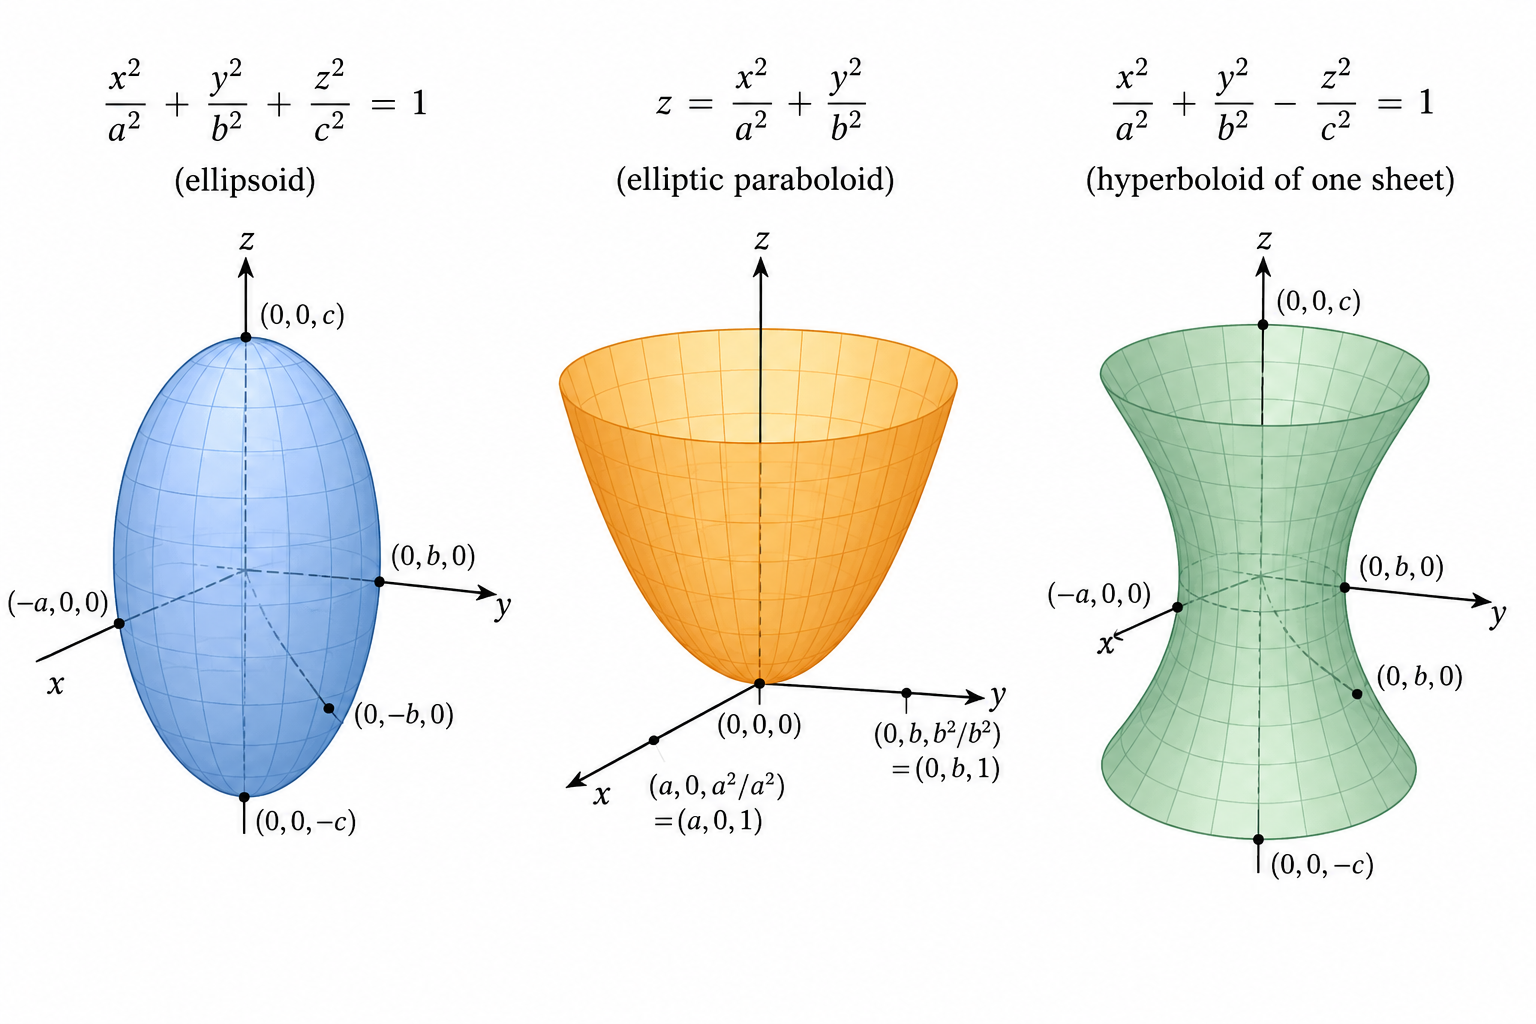
\includegraphics[width=\linewidth]{math_imgs/quadric_surface.png}
\end{minipage}

\paragraph{Vector Functions}

A vector-valued function has the following form, which describes a curve in space. 
\[
    \vect r(t)=\langle f(t),g(t),h(t)\rangle
\]
The derivative is componentwise, which is tangent to the curve.
\[
    \vect r'(t)=\langle f'(t),g'(t),h'(t)\rangle
\]
\[
    \frac{\dd}{\dd t}(\vect u\cdot\vect v)=\vect u'\cdot\vect v+\vect u\cdot\vect v'
\qquad
    \frac{\dd}{\dd t}(\vect u\times\vect v)=\vect u'\times\vect v+\vect u\times\vect v'
\]

\paragraph{Arc Length} The length of a smooth curve $\vect r(t)$ for $a\leq t\leq b$ is
\[
    L=\int_a^b \norm{\vect r'(t)}\dd t
\]
\paragraph{Curvature} Curvature measures how fast the tangent direction changes with respect to arc length:
\[
    \kappa=\left\lVert\frac{\dd \vect T}{\dd s}\right\rVert \qquad\vect T(t)=\frac{\vect r'(t)}{\norm{\vect r'(t)}}
\]
A practical formula is
\[
    \kappa(t)=\frac{\norm{\vect r'(t)\times \vect r''(t)}}{\norm{\vect r'(t)}^3}
\]
For a plane curve $y=f(x)$,
\[
    \kappa(x)=\frac{|f''(x)|}{\left(1+[f'(x)]^2\right)^{3/2}}
\]

\paragraph{Functions of Several Variables}
A function maps points in a domain to real numbers: $f(x,y)$ or $f(x,y,z)$. Its graph is the surface $z=f(x,y)$. A level curve $f(x,y)=c$ shows where the function has a constant value. A limit $\lim_{(x,y)\to(a,b)} f(x,y)=L$ exists if $f$ approaches $L$ along every path to $(a,b)$. A function is continuous at $(a,b)$ if $\lim_{(x,y)\to(a,b)}f(x,y)=f(a,b)$.

\paragraph{Partial Derivatives} These measure rates of change in the $x$ or $y$ direction:
\[
    f_x(x,y)=\lim_{h\to 0}\frac{f(x+h,y)-f(x,y)}{h}
\qquad
    f_y(x,y)=\lim_{h\to 0}\frac{f(x,y+h)-f(x,y)}{h}
\]



\paragraph{Linear Approximation} For $z=f(x,y)$, the tangent plane is the linear approximation:
\[
    z=f(a,b)+f_x(a,b)(x-a)+f_y(a,b)(y-b)
\]
\[
    f(x,y)\approx f(a,b)+f_x(a,b)(x-a)+f_y(a,b)(y-b)
\]

\paragraph{Chain Rule}

For a composition $z=f(x(t),y(t))$, the chain rule is
\[
    \frac{\dd z}{\dd t}=f_x\frac{\dd x}{\dd t}+f_y\frac{\dd y}{\dd t}
\]
For $z=f(x(s,t),y(s,t))$,
\[
    \pd{z}{s}=f_x\pd{x}{s}+f_y\pd{y}{s}
    \qquad
    \pd{z}{t}=f_x\pd{x}{t}+f_y\pd{y}{t}
\]

\defn{Directional Derivatives}{
Let \(f:\mathbb R^n\to\mathbb R\), \(\mathbf a\in\mathbb R^n\), \(\mathbf u\in\mathbb R^n\), $\norm{\mathbf{u}}=1$. The directional derivative of \(f\)
at \(\mathbf a\) in the direction \(\mathbf u\) is defined by
\[
    D_{\mathbf u}f(\mathbf a)
    =
    \lim_{h\to 0}
    \frac{f(\mathbf a+h\mathbf u)-f(\mathbf a)}{h}
\]}

\defn{Gradient}{
Let \(f:\mathbb R^n\to\mathbb R\) be differentiable at a point
\(\mathbf a=(a_1,\dots,a_n)\in\mathbb R^n\). The gradient of \(f\) at
\(\mathbf a\) is:
\[
    \nabla f(\mathbf a)
    =
    \left\langle
    \frac{\partial f}{\partial x_1}(\mathbf a),
    \frac{\partial f}{\partial x_2}(\mathbf a),
    \dots,
    \frac{\partial f}{\partial x_n}(\mathbf a)
    \right\rangle
\]
}
\noindent The gradient of $f$ at $\mathbf{a}$ is the vector of partial derivatives, and for any unit vector $\vect u$ the directional derivative in the direction of $\vect u$ is given by the dot product of the gradient with $\vect u$:
\[
    D_{\vect u}f(a,b)=\grad f(a,b)\cdot \vect u
\]

\begin{proof}
\noindent Let \(\mathbf u=\langle u_1,u_2\rangle\) be a unit vector. Since \(f\) is
differentiable at \((a,b)\), for \((\Delta x,\Delta y)\to(0,0)\),
\[
f(a+\Delta x,b+\Delta y)
=
f(a,b)+f_x(a,b)\Delta x+f_y(a,b)\Delta y
+o\!\left(\sqrt{(\Delta x)^2+(\Delta y)^2}\right)
\]
Take \(\Delta x=hu_1\) and \(\Delta y=hu_2\). Since \(\|\mathbf u\|=1\),
\[
f(a+hu_1,b+hu_2)
=
f(a,b)+h f_x(a,b)u_1+h f_y(a,b)u_2+o(|h|)
\]
Therefore,
\[
\begin{aligned}
D_{\mathbf u}f(a,b)
&=
\lim_{h\to 0}
\frac{f(a+hu_1,b+hu_2)-f(a,b)}{h} \\
&=
\lim_{h\to 0}
\left(
f_x(a,b)u_1+f_y(a,b)u_2+\frac{o(|h|)}{h}
\right) \\
&=
f_x(a,b)u_1+f_y(a,b)u_2 \\
&=
\nabla f(a,b)\cdot \mathbf u
\end{aligned}
\]
\end{proof}
\noindent The gradient points in the direction of \textbf{steepest ascent}, and the
maximum possible directional derivative is
$
    \|\nabla f(\mathbf a)\|.
$
Thus, \(\nabla f(\mathbf a)\) gives both the direction and the rate of fastest
increase of \(f\) at \(\mathbf a\).

\begin{proof}
\noindent Assume \(f\) is differentiable at \(\mathbf a\). Then for any $\norm{\mathbf{u}}=1$,
$
    D_{\mathbf u}f(\mathbf a)
    =
    \nabla f(\mathbf a)\cdot \mathbf u.
$
By the Cauchy--Schwarz inequality,
$
    \nabla f(\mathbf a)\cdot \mathbf u
    \leq
    \|\nabla f(\mathbf a)\|\,\|\mathbf u\|
    =
    \|\nabla f(\mathbf a)\|.
$
Equality holds when
$
    \mathbf u
    =
    \frac{\nabla f(\mathbf a)}{\|\nabla f(\mathbf a)\|},
$
provided \(\nabla f(\mathbf a)\neq \mathbf 0\).
\end{proof}

\defn{Jacobian Matrix}{
Let \(F:\mathbb R^n\to\mathbb R^m\) be a function. If all first-order partial derivatives of \(F_1,\dots,F_m\) exist at
\(\mathbf a\in\mathbb R^n\), then the Jacobian matrix of \(F\) at \(\mathbf a\)
is the \(m\times n\) matrix
\[
    J_F(\mathbf a)
    =
    \begin{bmatrix}
    \dfrac{\partial F_1}{\partial x_1}(\mathbf a)
    &
    \dfrac{\partial F_1}{\partial x_2}(\mathbf a)
    &
    \cdots
    &
    \dfrac{\partial F_1}{\partial x_n}(\mathbf a)
    \\[0.8em]
    \dfrac{\partial F_2}{\partial x_1}(\mathbf a)
    &
    \dfrac{\partial F_2}{\partial x_2}(\mathbf a)
    &
    \cdots
    &
    \dfrac{\partial F_2}{\partial x_n}(\mathbf a)
    \\
    \vdots & \vdots & \ddots & \vdots
    \\[0.4em]
    \dfrac{\partial F_m}{\partial x_1}(\mathbf a)
    &
    \dfrac{\partial F_m}{\partial x_2}(\mathbf a)
    &
    \cdots
    &
    \dfrac{\partial F_m}{\partial x_n}(\mathbf a)
    \end{bmatrix}  =
    \left[
    \frac{\partial F_i}{\partial x_j}(\mathbf a)
    \right]_{1\leq i\leq m,\;1\leq j\leq n} \quad  
    F(\mathbf x)
    =
    \begin{bmatrix}
    F_1(\mathbf x)\\
    F_2(\mathbf x)\\
    \vdots\\
    F_m(\mathbf x)
    \end{bmatrix} \quad
    \mathbf x=(x_1,\dots,x_n) 
\]
}

\defn{Hessian Matrix}{
Let \(f:\mathbb R^n\to\mathbb R\) be a scalar-valued function, where
$
    \mathbf x=(x_1,\dots,x_n).
$
If all second-order partial derivatives of \(f\) exist at
\(\mathbf a\in\mathbb R^n\), then the Hessian matrix of \(f\) at \(\mathbf a\)
is the \(n\times n\) matrix
\[
    H_f(\mathbf a)
    =
    \begin{bmatrix}
    \dfrac{\partial^2 f}{\partial x_1^2}(\mathbf a)
    &
    \dfrac{\partial^2 f}{\partial x_1\partial x_2}(\mathbf a)
    &
    \cdots
    &
    \dfrac{\partial^2 f}{\partial x_1\partial x_n}(\mathbf a)
    \\[0.8em]
    \dfrac{\partial^2 f}{\partial x_2\partial x_1}(\mathbf a)
    &
    \dfrac{\partial^2 f}{\partial x_2^2}(\mathbf a)
    &
    \cdots
    &
    \dfrac{\partial^2 f}{\partial x_2\partial x_n}(\mathbf a)
    \\
    \vdots & \vdots & \ddots & \vdots
    \\[0.4em]
    \dfrac{\partial^2 f}{\partial x_n\partial x_1}(\mathbf a)
    &
    \dfrac{\partial^2 f}{\partial x_n\partial x_2}(\mathbf a)
    &
    \cdots
    &
    \dfrac{\partial^2 f}{\partial x_n^2}(\mathbf a)
    \end{bmatrix}
    =
    \left[
    \frac{\partial^2 f}{\partial x_i\partial x_j}(\mathbf a)
    \right]_{1\leq i,j\leq n}
\]
}

\paragraph{Unconstrained Extrema}
Critical points satisfy $\grad f=\vect 0$.For a function of two variables, define
\[
    D=f_{xx}f_{yy}-(f_{xy})^2= |H_f|
\]
Then the second derivative test says:
\begin{itemize}
    \item if $D>0$ and $f_{xx}>0$, there is a local minimum;
    \item if $D>0$ and $f_{xx}<0$, there is a local maximum;
    \item if $D<0$, there is a saddle point;
    \item if $D=0$, the test is inconclusive.
\end{itemize}

\paragraph{Lagrange Multipliers}

To optimize $f(x,y)$ subject to $g(x,y)=c$, solve
\[
    \nabla f=\lambda\nabla g,
    \qquad g(x,y)=c
\]
For two constraints $g(x,y,z)=c$ and $h(x,y,z)=d$, solve
\[
    \nabla f=\lambda\nabla g+\mu\nabla h,
    \qquad g=c,
    \qquad h=d
\]
Evaluate $f$ at all candidate points, especially when the constraint set is closed and bounded.

\section{Multiple Integrals and Coordinate Systems}

\paragraph{Double Integrals}

For a function $f(x,y)$ over a rectangle $R=[a,b]\times[c,d]$, the double integral is
\[
    \iint_R f(x,y)\dd A
\]
It gives the signed volume under $z=f(x,y)$ over $R$. Fubini's theorem allows computation by iterated integrals:
\[
    \iint_R f(x,y)\dd A
    =\int_a^b\int_c^d f(x,y)\dd y\dd x
    =\int_c^d\int_a^b f(x,y)\dd x\dd y
\]
For a general region $D$, one writes the bounds according to the shape of the domain. A Type I region has
\[
    D=\{(x,y): a\leq x\leq b,\; g_1(x)\leq y\leq g_2(x)\}
\qquad
    \iint_D f\dd A=\int_a^b\int_{g_1(x)}^{g_2(x)}f(x,y)\dd y\dd x
\]
A Type II region has
\[
    D=\{(x,y): c\leq y\leq d,\; h_1(y)\leq x\leq h_2(y)\}
\qquad
    \iint_D f\dd A=\int_c^d\int_{h_1(y)}^{h_2(y)}f(x,y)\dd x\dd y
\]
Polar coordinates are $x=r\cos\theta, y=r\sin\theta$, with area element $\dd A=r\dd r\dd\theta$. Thus
\[
    \iint_D f(x,y)\dd A
    =\int_{\alpha}^{\beta}\int_{r_1(\theta)}^{r_2(\theta)}
    f(r\cos\theta,r\sin\theta)r\dd r\dd\theta
\]

\paragraph{Triple Integrals}

A triple integral over a solid region $E$ is
\[
    \iiint_E f(x,y,z)\dd V.
\]
It can represent mass when $f$ is density. Rectangular coordinates use
$
\dd V=\dd x\dd y\dd z
$.
Cylindrical coordinates are
$
    x=r\cos\theta,
    y=r\sin\theta,
    z=z
$
with
$\dd V=r\dd z\dd r\dd\theta$. Spherical coordinates are
$
    x=\rho\sin\phi\cos\theta,
    y=\rho\sin\phi\sin\theta,
    z=\rho\cos\phi
$,
with volume element
$
    \dd V=\rho^2\sin\phi\dd\rho\dd\phi\dd\theta
$.

\paragraph{Vector Field} A vector field assigns a vector to each point:
\[
    \vect F(x,y)=P(x,y)\vect i+Q(x,y)\vect j
\]

\paragraph{Line Integral}
For a scalar function $f$ or a vector field $\vect F$ along a curve $C$ parametrized by $\vect r(t)$, $a\leq t\leq b$,
\[
    \int_C f\dd s=\int_a^b f(\vect r(t))\norm{\vect r'(t)}\dd t
\]
\[
    \int_C \vect F\cdot \dd \vect r
    =\int_a^b \vect F(\vect r(t))\cdot \vect r'(t)\dd t
\]
The fundamental theorem for line integrals says that if $\vect F=\grad f$ is conservative, then:
\[
    \int_C \vect F\cdot \dd\vect r=f(\vect r(b))-f(\vect r(a))
\]


\begin{theorem}[Green's theorem]
Let $C$ be a positively oriented, piecewise smooth, simple closed curve enclosing a region $D$. If $P$ and $Q$ have continuous partial derivatives on an open region containing $D$, then
\[
    \oint_C P\dd x+Q\dd y
    =\iint_D\left(\pd{Q}{x}-\pd{P}{y}\right)\dd A
\]
\end{theorem}

\paragraph{Parametric Surface}

A parametric surface is described by
\[
    \vect r(u,v)=\langle x(u,v),y(u,v),z(u,v)\rangle,
    \qquad (u,v)\in D
\]
For fixed $u$ or fixed $v$, one obtains parameter curves on the surface. The tangent vectors are
$
    \vect r_u=\pd{\vect r}{u},
    \vect r_v=\pd{\vect r}{v}
$.
A normal vector is
$
    \vect r_u\times \vect r_v
$.
The tangent plane at $(u_0,v_0)$ is determined by the point $\vect r(u_0,v_0)$ and the normal vector
$
    \vect r_u(u_0,v_0)\times \vect r_v(u_0,v_0)
$. The surface area is
\[
    A(S)=\iint_D \norm{\vect r_u\times \vect r_v}\dd A
\]

\paragraph{Surface Integral}
For a scalar function $f$ over a parametric surface $S$ given by $\vect r(u,v)$
\[
    \iint_S f\dd S
    =\iint_D f(\vect r(u,v))\norm{\vect r_u\times\vect r_v}\dd A
\]
For a vector field $\vect F$, the flux across an oriented surface $S$ is
\[
    \iint_S \vect F\cdot \dd\vect S
    =\iint_D \vect F(\vect r(u,v))\cdot(\vect r_u\times\vect r_v)\dd A
\]

\begin{theorem}[Divergence theorem]
Let $E$ be a solid region with positively oriented closed boundary surface $S=\partial E$. Then
\[
    \iint_S \vect F\cdot\dd\vect S
    =\iiint_E \diver \vect F\dd V.
\]
\end{theorem}







% \chapter{Ordinary Differential Equations}

% \section{Introduction to Differential Equations}

% \subsection{Definitions and Terminology}

% \defn{Differential Equation}{
%     A \emph{differential equation} is an equation that contains derivatives of one
%     or more unknown functions with respect to one or more independent variables.
%     The unknown function is usually called the \emph{dependent variable}, and the
%     variable with respect to which differentiation is taken is called the
%     \emph{independent variable}.
% }

% \paragraph{Ordinary and Partial Differential Equations}{
%     A DE is called an \emph{ordinary differential equation}
%     (ODE) if it contains only ordinary derivatives with respect to a single
%     independent variable. It is called a \emph{partial differential equation}
%     (PDE) if it contains partial derivatives of one or more unknown functions of
%     two or more independent variables.
% }

% \ex{
%     The equations $\frac{dy}{dx}+5y=e^x$ and $\frac{d^2y}{dx^2}-6y=0$ are ordinary differential equations.  \\
%     By contrast, $\frac{\partial u}{\partial x} + \frac{\partial u}{\partial y} = 0$ is a partial differential equation.
% }

% \paragraph{Order.}
% The \emph{order} of a differential equation is the order of the highest derivative
% appearing in the equation. In one dependent variable, the general form of an
% $n$th-order ODE is
% \[
%     F(x,y,y',\ldots,y^{(n)})=0
% \]
% If the equation can be solved for the highest derivative, it can be written in
% \emph{normal form}:
% \[
%     \frac{d^n y}{dx^n} = f(x,y,y',\ldots,y^{(n-1)})
% \]

% \paragraph{Linear Ordinary Differential Equation}{
%     An $n$th-order ODE is \emph{linear} if it's linear in the dependent
%     variable and all of its derivatives. Its general form is
%     \[
%         a_n(x)y^{(n)}
%         +a_{n-1}(x)y^{(n-1)}
%         +\cdots
%         +a_1(x)y'
%         +a_0(x)y
%         =
%         g(x)
%     \]
%     The coefficients may depend on the independent variable $x$, but not on
%     $y$ or its derivatives.
% }

% \ex{
%     The equation $y''-2y'+y=e^x$ is linear. \\
%     The equations $yy'+x=0$, $y''+\sin y=0$ and $(y')^2+y=0$ are nonlinear. 
% }

% \paragraph{Solution of an ODE}{
%     A function $\phi$, defined on an interval $I$ and possessing the required
%     derivatives on $I$, is called a \emph{solution} of an $n$th-order ODE if
%     substituting $y=\phi(x)$ into the equation reduces it to an identity on $I$.
% }

% \paragraph{Interval of Definition}{
%     The interval on which a solution is defined is called the \emph{interval of
%     definition}, \emph{interval of existence}, \emph{interval of validity}, or
%     \emph{domain of the solution}.
% }

% \paragraph{Explicit and Implicit Solutions}{
%     An \emph{explicit solution} expresses the dependent variable directly as a
%     function of the independent variable: $y=\phi(x)$. An \emph{implicit solution} is a relation $ G(x,y)=0$ that defines at least one differentiable function $y=\phi(x)$ satisfying the differential equation on an interval.
% }

% \ex{
%     The relation $x^2+y^2=25$ is an implicit solution of $\frac{dy}{dx}=-\frac{x}{y}$. On the interval $(-5,5)$, it gives two explicit branches: $y=\sqrt{25-x^2}$ and $y=-\sqrt{25-x^2}$. 
% }

% \paragraph{Families, Particular Solutions, and Singular Solutions}{
%     A solution containing one or more constants is called a
%     \emph{family of solutions}. A solution obtained by assigning values
%     to these constants is called a \emph{particular solution}. A \emph{singular solution} is a solution that can't be obtained from the family of solutions by any choice of the arbitrary constants.
% }

% \ex{
%     The equation $ y'=y$ has the one-parameter family of solutions $ y=ce^x$. If the condition $y(0)=3$ is imposed, then $c=3$, so the particular solution is $y=3e^x$. 
% }

% \paragraph{System of ODEs}{
%     A \emph{system of ordinary differential equations} consists of two or more
%     equations involving derivatives of two or more unknown functions of a single
%     independent variable. 
% }

% \subsection{Initial-Value Problems}

% \defn{Initial-Value Problem}{
%     An $n$th-order \emph{initial-value problem} consists of an $n$th-order
%     differential equation together with $n$ side conditions imposed at the same
%     point $x_0$:
%     \[
%         \frac{d^n y}{dx^n}
%         =
%         f(x,y,y',\ldots,y^{(n-1)})
%     \]
%     subject to
%     \[
%         y(x_0)=y_0,\qquad
%         y'(x_0)=y_1,\qquad
%         \ldots,\qquad
%         y^{(n-1)}(x_0)=y_{n-1}
%     \]
% }

% \thmr{Existence and Uniqueness for a First-Order IVP}{existenceuniqueness}{
%     Let $R$ be a rectangular region in the $xy$-plane containing the point
%     $(x_0,y_0)$. If $f(x,y)$ and $\dfrac{\partial f}{\partial y}(x,y)$ are
%     continuous on $R$, then there exists an interval $I_0=(x_0-h,x_0+h)$ for some $h>0$ on which the initial-value problem
%     \[
%         \frac{dy}{dx}=f(x,y),
%         \qquad
%         y(x_0)=y_0
%     \]
%     has a unique solution.
% }

% \rmk{
%     This theorem is local: it guarantees a unique solution only near \(x_0\), not
% necessarily on the largest possible interval. It gives sufficient, not necessary,
% conditions. Roughly, \(f\) continuous gives existence, and \(f_y\) continuous gives
% uniqueness.
% }

% \ex{
%     The initial-value problem $\frac{dy}{dx}=x\sqrt{y}, y(0)=0$ has more than one solution. For example, $y=0$ and $y=\frac{x^4}{16}$ both satisfy the differential equation and the initial condition. This does not contradict the existence--uniqueness theorem, because $\frac{\partial}{\partial y}\bigl(x\sqrt{y}\bigr) = \frac{x}{2\sqrt{y}}$ is not continuous at $y=0$.
% }

% \section{First-Order Differential Equations}

% \subsection{Solution Curves Without an Explicit Solution}

% \paragraph{Direction Field}{
%     Consider a first-order differential equation in normal form $\frac{dy}{dx}=f(x,y)$
%     At each point $(x,y)$ where $f$ is defined, the value $f(x,y)$ gives the slope
%     of a small line segment, called a \emph{lineal element}. A collection of such
%     lineal elements drawn on a grid in the $xy$-plane is called a
%     \emph{direction field}.
% }

% \defn{Autonomous First-Order Differential Equation}{
%     A first-order differential equation is called \emph{autonomous} if the
%     independent variable does not appear explicitly. In normal form, it can be
%     written as
%     \[
%         \frac{dy}{dx}=f(y)
%     \]
% }

% \paragraph{Critical Point and Equilibrium Solution}{
%     A real number $c$ is called a \emph{critical point}, \emph{equilibrium point}, or
%     \emph{stationary point} of $\frac{dy}{dx}=f(y)$ if $f(c)=0$. In this case, the constant function $y(x)=c$ is a solution, called an \emph{equilibrium solution}.
% }

% \paragraph{Phase Line and Phase Portrait}{
%     For an autonomous equation $\frac{dy}{dx}=f(y)$ a \emph{phase line} is a vertical line on which the critical points are marked. The sign of $f(y)$ on each interval between critical points determines whether solutions are increasing or decreasing. The resulting diagram is called a \emph{one-dimensional phase portrait}.
% }

% \paragraph{Attractors, Repellers, and Semi-Stable Points}{
%     Let $c$ be a critical point of $\frac{dy}{dx}=f(y)$
%     \begin{itemize}
%         \item If nearby solutions approach $c$ as $x\to\infty$, then $c$ is an
%         \emph{attractor} or \emph{asymptotically stable equilibrium}.
%         \item If nearby solutions move away from $c$, then $c$ is a \emph{repeller}
%         or \emph{unstable equilibrium}.
%         \item If solutions approach $c$ from one side and move away from $c$ from
%         the other side, then $c$ is \emph{semi-stable}.
%     \end{itemize}
% }

% \prop{
%     If $y(x)$ is a solution of the autonomous equation $\frac{dy}{dx}=f(y)$ then for any constant $k$, $y_1(x)=y(x-k)$ is also a solution. This is called the \emph{translation property.}
% }


% \subsection{Separable Equations}

% \defn{Separable Equation}{
%     A first-order differential equation of the form
%     \[
%         \frac{dy}{dx}=g(x)h(y)
%     \]
%     is called a \emph{separable differential equation}.
% }

% \paragraph{Procedure.}
% To solve a separable differential equation:
% \begin{enumerate}
%     \item Write the equation in separable form $\frac{dy}{dx}=g(x)h(y)$.
%     \item Assuming $h(y)\neq 0$, separate the variables $\frac{1}{h(y)}\,dy=g(x)\,dx$. 
%      \item Integrate both sides $\int \frac{1}{h(y)}\,dy=\int g(x)\,dx$. 
%     \item Write the solution implicitly as $ H(y)=G(x)+C$.
% \end{enumerate}

% \rmk{
%     When solving a separable equation, any value $r$ such that $h(r)=0$ should be
%     checked separately. The constant function $y=r$ may be a solution, but it may
%     be lost after division by $h(y)$.
% }


% \subsection{Linear Equations}

% \defn{First-Order Linear Equation}{
%     A first-order differential equation of the form $ a_1(x)\frac{dy}{dx}+a_0(x)y=g(x)$ is called a \emph{linear differential equation} in the dependent variable $y$.
%     If $a_1(x)\neq 0$, division by $a_1(x)$ gives the standard form
%     \[
%         \frac{dy}{dx}+P(x)y=f(x)
%     \]
% }

% \paragraph{Procedure.}
% To solve a first-order linear equation:
% \begin{enumerate}
%     \item Put the equation in standard form $\frac{dy}{dx}+P(x)y=f(x)$. 
%     \item Compute the integrating factor $\mu(x)=e^{\int P(x)\,dx}$. 
%     \item Multiply both sides by $\mu(x)$ and rewrite the left-hand side as $\frac{d}{dx}\bigl(\mu(x)y\bigr)$. 
%     \item Integrate both sides and solve for $y$.
%     \[
%     y=e^{-\int P(x)\,dx}
%     \left(
%         \int e^{\int P(x)\,dx}f(x)\,dx+C
%     \right)
%     \]
% \end{enumerate}



% \subsection{Exact Differential Equations}

% \defn{Exact Differential Equation}{
%     A first-order differential equation written in differential form
%     \[
%         M(x,y)\,dx+N(x,y)\,dy=0
%     \]
%     is called an \emph{exact equation} if there exists a function $\Phi(x,y)$ such
%     that
%     \[
%         \frac{\partial \Phi}{\partial x}=M(x,y),
%         \qquad
%         \frac{\partial \Phi}{\partial y}=N(x,y)
%     \]
%     In that case, $d\Phi=M\,dx+N\,dy$ and the solution is given implicitly by $\Phi(x,y)=C$.
% }

% \thmr{Criterion for Exactness}{exactnesscriterion}{
%     Suppose $M(x,y)$ and $N(x,y)$ have continuous first partial derivatives in a
%     rectangular region $R$. Then $M(x,y)\,dx+N(x,y)\,dy$
%     is an exact differential in $R$ if and only if
%     \[
%         \frac{\partial M}{\partial y}
%         =
%         \frac{\partial N}{\partial x}
%     \]
% }

% \paragraph{Procedure.}

% \begin{enumerate}
%     \item Integrate $M$ with respect to $x$: $ \Phi(x,y)=\int M(x,y)\,dx+g(y)$.
%     \item Differentiate this expression with respect to $y$: $\Phi_y=\frac{\partial}{\partial y}
%         \left(\int M(x,y)\,dx\right)+g'(y)$. 
%     \item Set $\Phi_y=N(x,y)$ and solve for $g'(y)$. Integrate to find $g(y)$.
%     \item Write the solution as $\Phi(x,y)=C$.
% \end{enumerate}

% \paragraph{Integrating Factors for Nonexact Equations.}
% If $M(x,y)\,dx+N(x,y)\,dy=0$ is not exact, it may become exact after multiplication by a nonzero function $\mu(x,y)$: $\mu M\,dx+\mu N\,dy=$. Two useful special cases are:
% \[
% \begin{cases}
%     \mu(x) =\exp\left( \int \frac{M_y-N_x}{N}\,dx \right), \qquad \text{if } \frac{M_y-N_x}{N} \text{ depends only on }x \\
%     \mu(y)
%     =
%     \exp\left(
%         \int \frac{N_x-M_y}{M}\,dy
%     \right),
%     \qquad
%     \text{if }
%     \frac{N_x-M_y}{M}
%     \text{ depends only on }y
% \end{cases}
% \]


% \subsection{Solutions by Substitutions}

% \defn{Substitution Method}{
%     For a first-order equation $\frac{dy}{dx}=f(x,y)$ introduce a substitution $y=g(x,u), u=u(x)$. By the chain rule,
%     \[
%         \frac{dy}{dx}
%         =
%         \frac{\partial g}{\partial x}(x,u)
%         +
%         \frac{\partial g}{\partial u}(x,u)\frac{du}{dx}
%     \]
%     After substitution, the original equation may become a simpler equation $\frac{du}{dx}=F(x,u)$. If this new equation is separable or linear, it can be solved by earlier methods. Finally, substitute back to obtain $y$.
% }

% \paragraph{Solving a Homogeneous Equation.}
% If the equation is homogeneous, use the substitution
% \[
%     y=ux,
%     \qquad
%     \frac{dy}{dx}=u+x\frac{du}{dx}
% \]

% \paragraph{Solving a Bernoulli Equation.}{
%     A differential equation of the form $\frac{dy}{dx}+P(x)y=f(x)y^n$ is called a \emph{Bernoulli equation}. For $n\neq 0,1$, it can be reduced to a linear equation by the substitution
%     \[
%         u=y^{1-n}, \qquad  \frac{du}{dx}
%     =
%     (1-n)y^{-n}\frac{dy}{dx}
%     \]
% }

% \paragraph{Reduction to Separation of Variables}{
%     A differential equation of the form $\frac{dy}{dx}=f(Ax+By+C),B\neq 0$ can be reduced to a separable equation by the substitution
%     \[
%         u=Ax+By+C,\qquad \frac{du}{dx}=A+B\frac{dy}{dx}
%     \]
% }


% \subsection{A Numerical Method}

% \defn{Euler's Method}{
%     Consider the initial-value problem $y'=f(x,y), y(x_0)=y_0$, Euler's method approximates the solution by repeatedly following tangent lines: 
%     \[
%     x_n=x_0+nh,
%     \qquad
%     y_{n+1}=y_n+h f(x_n,y_n),
%     \qquad
%     n=0,1,2,\ldots
%     \]
% }

% \section{Higher-Order Differential Equations}

% \subsection{Theory of Linear Equations}

% \paragraph{Linear $n$th-Order Differential Equation}{
%     A linear $n$th-order differential equation has the form
%     \[
%         a_n(x)y^{(n)}+a_{n-1}(x)y^{(n-1)}+\cdots+a_1(x)y'+a_0(x)y=g(x)
%     \]
%     where $a_n(x)\neq 0$ on an interval $I$. If $g(x)=0$, the equation is
%     \emph{homogeneous}; otherwise it is \emph{nonhomogeneous}. An $n$th-order initial-value problem specifies the value of $y$ and its first
%     $n-1$ derivatives at the same point $x_0$:
%     \[
%         y(x_0)=y_0,\qquad
%         y'(x_0)=y_1,\qquad
%         \ldots,\qquad
%         y^{(n-1)}(x_0)=y_{n-1}
%     \]
% }

% \thmr{Existence and Uniqueness for Linear IVPs}{higherorderexistence}{
%     Suppose $a_n,a_{n-1},\ldots,a_0$ and $g$ are continuous on an interval $I$, and
%     $a_n(x)\neq 0$ for every $x\in I$. Then for any $x_0\in I$, the corresponding
%     $n$th-order linear initial-value problem has a unique solution on $I$.
% }

% \rmk{
%     This theorem is much stronger than the first-order local theorem: for linear
%     equations, the solution exists on the whole interval on which the coefficient
%     functions are continuous and the leading coefficient is nonzero.
% }

% \paragraph{Boundary-Value Problems.}
% A boundary-value problem imposes conditions at different points, for example $y(a)=y_0, y(b)=y_1$. Unlike initial-value problems, a boundary-value problem may have infinitely many
% solutions, exactly one solution, or no solution.

% \paragraph{Differential Operator Notation.}
% Let $D=\frac{d}{dx}$. Then $D^n y=\frac{d^n y}{dx^n}$. The linear differential operator is
% \[
%     L=a_n(x)D^n+a_{n-1}(x)D^{n-1}+\cdots+a_1(x)D+a_0(x)
% \]
% so the differential equation can be written compactly as $L[y]=g(x)$. 

% \prop{
%     The operator $L$ is linear, where $\alpha$ and $\beta$ are constants:
%     \[
%         L[\alpha f+\beta g]=\alpha L[f]+\beta L[g],
%     \]
% }

% \thmr{Superposition Principle for Homogeneous Equations}{homogeneoussuperposition}{
%     If $y_1,\ldots,y_k$ are solutions of the homogeneous equation $L[y]=0$ on an
%     interval $I$, then every linear combination $y=c_1y_1+\cdots+c_ky_k$ is also a solution on $I$.
% }

% \defn{Linear Independence and the Wronskian}{
%     Functions $f_1,\ldots,f_n$ are linearly dependent on $I$ if there exist
%     constants $c_1,\ldots,c_n$, not all zero, such that
%     \[
%         c_1f_1(x)+\cdots+c_nf_n(x)=0
%     \]
%     for every $x\in I$. Otherwise they are linearly independent. The \emph{Wronskian} of $f_1,\ldots,f_n$ is
%     \[
%         W(f_1,\ldots,f_n)=
%         \begin{vmatrix}
%             f_1 & f_2 & \cdots & f_n\\
%             f_1' & f_2' & \cdots & f_n'\\
%             \vdots & \vdots & & \vdots\\
%             f_1^{(n-1)} & f_2^{(n-1)} & \cdots & f_n^{(n-1)}
%         \end{vmatrix}
%     \]
% }

% \paragraph{Wronskian Criterion for Solutions}{wronskiancriterion}{
%     Let $y_1,\ldots,y_n$ be $n$ solutions of a homogeneous linear $n$th-order
%     differential equation on $I$. Then they are linearly independent on $I$ if and
%     only if for every $x\in I$: 
%     \[
%         W(y_1,\ldots,y_n)(x)\neq 0
%     \]
% }

% \paragraph{Fundamental Set of Solutions}{
%     A set of $n$ linearly independent solutions of a homogeneous linear
%     $n$th-order differential equation is called a \emph{fundamental set of
%     solutions}.
% }

% \thmr{General Solution of a Homogeneous Linear Equation}{homogeneousgeneralsolution}{
%     If $y_1,\ldots,y_n$ form a fundamental set of solutions for $L[y]=0$ on $I$,
%     then the general solution is
%     \[
%         y=c_1y_1+\cdots+c_ny_n
%     \]
% }

% \thmr{General Solution of a Nonhomogeneous Linear Equation}{nonhomogeneousgeneralsolution}{
%     If $y_p$ is one particular solution of $L[y]=g(x)$ and
%     $y_c=c_1y_1+\cdots+c_ny_n$ is the general solution of the associated
%     homogeneous equation $L[y]=0$, then the general solution of the
%     nonhomogeneous equation is
%     \[
%         y=y_c+y_p
%     \]
% }

% \prop{
%     If $y_{p1},\ldots,y_{pk}$ are particular solutions of
%     \[
%         L[y]=g_1(x),\qquad \ldots,\qquad L[y]=g_k(x)
%     \]
%     then $y_p=y_{p1}+\cdots+y_{pk}$ is a particular solution of
%     \[
%         L[y]=g_1(x)+\cdots+g_k(x)
%     \]
% }

% \subsection{Reduction of Order}

% \thmr{Reduction of Order Formula}{reductionoforder}{
%     Let $y_1(x)$ be a nonzero solution of
%     \[
%         y''+P(x)y'+Q(x)y=0
%     \]
%     on an interval $I$. Then a second solution is
%     \[
%         y_2(x)=y_1(x)\int
%         \frac{e^{-\int P(x)\,dx}}{[y_1(x)]^2}\,dx
%     \]
% }

% \paragraph{Procedure.}
% \begin{enumerate}
%     \item Put the equation in standard form $y''+P(x)y'+Q(x)y=0$.
%     \item Identify a known nonzero solution $y_1$.
%     \item Use $y_2=y_1\int \frac{e^{-\int P(x)\,dx}}{y_1^2}\,dx$. 
%     \item Write the general solution as $y=c_1y_1+c_2y_2$.
% \end{enumerate}


% \subsection{Homogeneous Linear Equations with Constant Coefficients}

% \paragraph{Auxiliary Equation.}
% For $a_ny^{(n)}+a_{n-1}y^{(n-1)}+\cdots+a_1y'+a_0y=0$, try $y=e^{mx}$. Substitution gives the \emph{auxiliary equation} $a_nm^n+a_{n-1}m^{n-1}+\cdots+a_1m+a_0=0$. The roots of this polynomial determine the solution.

% \paragraph{Second-Order Case.}
% For $ay''+by'+cy=0$ the auxiliary equation is $am^2+bm+c=0$.

% \begin{center}
% \begin{tabular}{c|c}
% Root type & General solution\\
% \hline
% $m_1\neq m_2$ real & $y=c_1e^{m_1x}+c_2e^{m_2x}$\\[0.3em]
% $m_1=m_2=m$ & $y=c_1e^{mx}+c_2xe^{mx}$\\[0.3em]
% $m=\alpha\pm i\beta$ & $y=e^{\alpha x}\bigl(c_1\cos \beta x+c_2\sin \beta x\bigr)$
% \end{tabular}
% \end{center}

% \paragraph{Higher-Order Roots.}
% If $m$ is a real root of multiplicity $k$, then the corresponding solutions are
% \[
%     e^{mx},\quad xe^{mx},\quad x^2e^{mx},\quad \ldots,\quad x^{k-1}e^{mx}
% \]
% If $\alpha\pm i\beta$ is a complex conjugate pair of multiplicity $k$, then the
% real solutions are
% \[
%     e^{\alpha x}\cos \beta x,\quad xe^{\alpha x}\cos \beta x,
%     \quad \ldots,\quad x^{k-1}e^{\alpha x}\cos \beta x
% \]
% \[
%     e^{\alpha x}\sin \beta x,\quad xe^{\alpha x}\sin \beta x,
%     \quad \ldots,\quad x^{k-1}e^{\alpha x}\sin \beta x
% \]

% \subsection{Undetermined Coefficients: Superposition Approach}

% \paragraph{When the Method Applies.}
% The method of undetermined coefficients applies to nonhomogeneous linear
% differential equations with constant coefficients, $a_ny^{(n)}+a_{n-1}y^{(n-1)}+\cdots+a_1y'+a_0y=g(x)$, when $g(x)$ is a finite sum of constants, polynomials, exponentials, sines, cosines, or products of these functions.

% \paragraph{Procedure.}
% \begin{enumerate}
%     \item Solve the associated homogeneous equation to find $y_c$.
%     \item Guess the form of a particular solution $y_p$ based on $g(x)$.
%     \item Substitute $y_p$ into the original equation and solve for the unknown coefficients.
%     \item Write the general solution as $y=y_c+y_p$.
% \end{enumerate}

% \paragraph{Common Trial Forms.}
% \begin{center}
% \begin{tabular}{c|c}
% $g(x)$ & Trial form for $y_p$\\
% \hline
% $k$ & $A$\\[0.2em]
% $a_mx^m+\cdots+a_0$ & $A_mx^m+\cdots+A_0$\\[0.2em]
% $e^{\alpha x}$ & $Ae^{\alpha x}$\\[0.2em]
% $x^me^{\alpha x}$ & $(A_mx^m+\cdots+A_0)e^{\alpha x}$\\[0.2em]
% $\cos \beta x$ or $\sin \beta x$ & $A\cos \beta x+B\sin \beta x$\\[0.2em]
% $e^{\alpha x}\cos \beta x$ or $e^{\alpha x}\sin \beta x$ &
% $e^{\alpha x}(A\cos \beta x+B\sin \beta x)$
% \end{tabular}
% \end{center}

% \rmk{If any term in the guessed $y_p$ is already contained in $y_c$, multiply the whole
% guess by the smallest power $x^s$ that removes the duplication: $y_p=x^s(\text{original guess})$.}

% \subsection{Undetermined Coefficients: Annihilator Approach}

% \defn{Annihilator}{
%     A differential operator $L$ with constant coefficients is called an
%     \emph{annihilator} of $f(x)$ if
%     \[
%         L[f(x)]=0
%     \]
% }

% \paragraph{Basic Annihilators.}
% \[
%     D^n \text{ annihilates } 1,x,x^2,\ldots,x^{n-1}.
% \]
% \[
%     (D-\alpha)^n \text{ annihilates }
%     e^{\alpha x},xe^{\alpha x},\ldots,x^{n-1}e^{\alpha x}.
% \]
% \[
%     \bigl[(D-\alpha)^2+\beta^2\bigr]^n
%     \text{ annihilates }
%     x^ke^{\alpha x}\cos\beta x
%     \text{ and }
%     x^ke^{\alpha x}\sin\beta x, k=0,1,\ldots,n-1.
% \]

% \paragraph{Procedure.}
% To solve $L[y]=g(x)$ by annihilators:
% \begin{enumerate}
%     \item Solve $L[y]=0$ to find the complementary function $y_c$.
%     \item Find an operator $L_1$ such that $L_1[g]=0$.
%     \item Apply $L_1$ to obtain the homogeneous equation $L_1L[y]=0$. 
%     \item Solve the higher-order homogeneous equation.
%     \item Remove the terms already in $y_c$; the remaining terms give the form of $y_p$.
%     \item Substitute into the original equation to determine the coefficients.
% \end{enumerate}

% \rmk{
%     The annihilator method justifies the guessing method. It is often more useful
%     for finding the correct form of $y_p$ than for doing the final coefficient
%     calculation.
% }

% \subsection{Variation of Parameters}

% \paragraph{Procedure.}
% \begin{enumerate}
%     \item Put the equation in standard form $y''+P(x)y'+Q(x)y=f(x)$.
%     \item Solve the homogeneous equation to find $y_1,y_2$.
%     \item Compute $W=y_1y_2'-y_2y_1'$. Compute $u_1'$ and $u_2'$ using $u_1'=-\frac{y_2f}{W}, u_2'=\frac{y_1f}{W}$
%     \item Integrate to find $u_1,u_2$, then write $y_p=u_1y_1+u_2y_2$.
%     \item The general solution is $y=y_c+y_p$.
% \end{enumerate}

% \subsection{Cauchy--Euler Equations}

% \defn{Cauchy--Euler Equation}{
%     A second-order Cauchy--Euler equation has the form where $a,b,c$ are constants:
%     \[
%         ax^2y''+bxy'+cy=g(x)
%     \]
%     More generally, an $n$th-order Cauchy--Euler
%     equation has powers of $x$ matched to the order of the derivative:
%     \[
%         a_nx^ny^{(n)}+a_{n-1}x^{n-1}y^{(n-1)}+
%         \cdots+a_1xy'+a_0y=g(x)
%     \]
% }

% \paragraph{Root Cases.}
% On an interval where $x>0$:
% \begin{center}
% \begin{tabular}{c|c}
% Root type & General solution\\
% \hline
% $m_1\neq m_2$ real & $y=c_1x^{m_1}+c_2x^{m_2}$\\[0.3em]
% $m_1=m_2=m$ & $y=c_1x^m+c_2x^m\ln x$\\[0.3em]
% $m=\alpha\pm i\beta$ &
% $y=x^\alpha\bigl(c_1\cos(\beta\ln x)+c_2\sin(\beta\ln x)\bigr)$
% \end{tabular}
% \end{center}

% \paragraph{Nonhomogeneous Case.}
% \begin{enumerate}
%     \item Solve the associated homogeneous Cauchy--Euler equation.
%     \item Divide by the leading coefficient to put the equation in standard form.
%     \item Use variation of parameters to find $y_p$.
% \end{enumerate}

% \subsection{Solving Systems of Linear Differential Equations by Elimination}

% \defn{Solution of a System}{
%     A solution of a system of differential equations is a set of sufficiently
%     differentiable functions, such as
%     \[
%         x=\Phi_1(t),\qquad y=\Phi_2(t),\qquad z=\Phi_3(t)
%     \]
%     that satisfies every equation in the system on a common interval $I$.
% }

% \paragraph{Procedure.}
% \begin{enumerate}
%     \item Rewrite the system using the differential operator $D$.
%     \item Apply operators to the equations so that one unknown can be eliminated.
%     \item Solve the resulting higher-order equation for one dependent variable.
%     \item Substitute back into one original equation to find the other variables.
%     \item Use the original system to relate the arbitrary constants.
% \end{enumerate}

% \section{Series Solutions of Linear Equations}

% \subsection{Review of Power Series}

% \defn{Power Series}{
%     A \emph{power series centered at $a$} is an infinite series of the form
%     \[
%         \sum_{n=0}^{\infty} c_n(x-a)^n
%         =
%         c_0+c_1(x-a)+c_2(x-a)^2+\cdots
%     \]
% }

% \paragraph{Convergence and Radius of Convergence.}
% A power series may converge for some values of $x$ and diverge for others. The set
% of all real numbers $x$ for which the series converges is called its
% \emph{interval of convergence}. There is a number $R$, called the
% \emph{radius of convergence}, such that
% $
%     \sum_{n=0}^{\infty} c_n(x-a)^n
%     \text{converges for } |x-a|<R
% $
% and diverges for $|x-a|>R$. At the endpoints $x=a\pm R$, convergence must be
% checked separately.

% \paragraph{Ratio Test.}
% For a power series, the ratio test often gives the radius of convergence. If
% $
%     L
%     =
%     \lim_{n\to\infty}
%     \left|
%         \frac{c_{n+1}(x-a)^{n+1}}{c_n(x-a)^n}
%     \right|
% $
% then the series converges absolutely when $L<1$ and diverges when $L>1$.
% The test is inconclusive when $L=1$, which usually corresponds to the endpoints.

% \defn{Analytic Function}{
%     A function $f$ is \emph{analytic at $a$} if it can be represented by a power
%     series centered at $a$ with $R>0$:
%     \[
%         f(x)=\sum_{n=0}^{\infty} c_n(x-a)^n
%     \]
% }

% \prop{
%     If $\sum_{n=0}^{\infty} c_n(x-a)^n=0$ for all $x$ in some open interval around $a$, then every coefficient must be
%     zero: $c_n=0, n=0,1,2,\ldots$. This is called the \emph{identity property} of power series.
% }


% \subsection{Solutions About Ordinary Points}

% \defn{Ordinary and Singular Points}{
%     Consider the homogeneous linear second-order equation $a_2(x)y''+a_1(x)y'+a_0(x)y=0$. After division by $a_2(x)$, write it in standard form $y''+P(x)y'+Q(x)y=0$. A point $x=x_0$ is an \emph{ordinary point} if both $P(x)$ and $Q(x)$ are
%     analytic at $x_0$. Otherwise, $x=x_0$ is a \emph{singular point}.
% }

% \thmr{Existence of Power Series Solutions}{powerseriesordinary}{
%     If $x=x_0$ is an ordinary point of $a_2(x)y''+a_1(x)y'+a_0(x)y=0$ then the equation has two linearly independent solutions of the form $y=\sum_{n=0}^{\infty} c_n(x-x_0)^n$. Each power series solution converges at least for $|x-x_0|<R$ where $R$ is the distance from $x_0$ to the nearest singular point.
% }

% \paragraph{Procedure.}
% To find a power series solution about an ordinary point:
% \begin{enumerate}
%     \item Assume $ y=\sum_{n=0}^{\infty} c_n(x-x_0)^n$.
%     \item Differentiate term by term to find $y'$ and $y''$. Substitute $y,y',y''$ into the differential equation. Make all series use the same power of $x-x_0$. Set each coefficient equal to zero. Solve the resulting recurrence relation. 
%     \item Write the solution in terms of the arbitrary constants, usually $c_0$ and $c_1$.
% \end{enumerate}


% \subsection{Solutions About Singular Points}

% \defn{Regular and Irregular Singular Points}{
%     Suppose $x=x_0$ is a singular point of $y''+P(x)y'+Q(x)y=0$. Then $x=x_0$ is a \emph{regular singular point} if
%     \[
%         p(x)=(x-x_0)P(x),
%         \qquad
%         q(x)=(x-x_0)^2Q(x)
%     \]
%     are both analytic at $x_0$. A singular point that is not regular is called an
%     \emph{irregular singular point}.
% }

% \thmr{Frobenius' Theorem}{frobeniustheorem}{
%     If $x=x_0$ is a regular singular point of $a_2(x)y''+a_1(x)y'+a_0(x)y=0$, then there exists at least one solution of the following form  where $r$ is a constant determined by the differential equation
%     \[
%         y
%         =
%         \sum_{n=0}^{\infty} c_n(x-x_0)^{n+r}
%         =
%         (x-x_0)^r
%         \sum_{n=0}^{\infty} c_n(x-x_0)^n,
%         \qquad c_0\neq 0
%     \]
% }

% \paragraph{Indicial Equation.}
% For a regular singular point at $x=0$, write $ y''+P(x)y'+Q(x)y=0$, and define
% \[
%     p(x)=xP(x)=a_0+a_1x+a_2x^2+\cdots,
%     \qquad
%     q(x)=x^2Q(x)=b_0+b_1x+b_2x^2+\cdots
% \]
% Then the \emph{indicial equation} is $r(r-1)+a_0r+b_0=0$. Its roots are called the \emph{indicial roots}.

% \paragraph{Procedure.}
% To solve near a regular singular point $x=0$:
% \begin{enumerate}
%     \item Assume a Frobenius solution $y=\sum_{n=0}^{\infty} c_nx^{n+r},
%         c_0\neq 0$.
%     \item Compute $y'$ and $y''$. Substitute into the differential equation. Set the coefficient of the lowest power of $x$ equal to zero. This gives the indicial equation. Solve the recurrence relation for each indicial root.
%     \item Determine whether one or two linearly independent Frobenius series are obtained.
% \end{enumerate}

% \paragraph{Three Cases for Indicial Roots.}
% Assume $r_1$ and $r_2$ are real indicial roots with $r_1\ge r_2$.

% \begin{center}
% \begin{tabular}{c|c}
% Case & Form of solutions\\
% \hline
% $r_1-r_2\notin \mathbb{Z}_{>0}$ &
% Two Frobenius series usually exist\\[0.4em]
% $r_1-r_2\in \mathbb{Z}_{>0}$ &
% One Frobenius series always exists; the second may contain $\ln x$\\[0.4em]
% $r_1=r_2$ &
% Second solution contains $\ln x$
% \end{tabular}
% \end{center}
% More explicitly $ y_1=\sum_{n=0}^{\infty} c_nx^{n+r_1}, c_0\neq 0$. The second solution may have the form
% \[
%     y_2=C y_1\ln x+\sum_{n=0}^{\infty} b_nx^{n+r_2},
%     \qquad b_0\neq 0,
% \]
% where $C$ may be zero in the second case, but is nonzero in the repeated-root case.


% \section{The Laplace Transform}

% \subsection{Definition of the Laplace Transform}

% \defn{Laplace Transform}{
%     Let $f$ be defined for $t\ge 0$. The \emph{Laplace transform} of $f$ is
%     \[
%         \mathcal{L}\{f(t)\}=F(s)=\int_0^\infty e^{-st}f(t)\,dt 
%         =
%         \lim_{b\to\infty}\int_0^b e^{-st}f(t)\,dt
%     \]
%     The variable $t$ is the original variable, while $s$ is the transform variable.
% }

% \paragraph{Basic Transform Table.}
% For suitable values of $s$,
% \[
% \begin{array}{c|c}
%     f(t) & \mathcal{L}\{f(t)\}=F(s)\\
%     \hline
%     1 & \dfrac{1}{s}\\[0.7em]
%     t^n & \dfrac{n!}{s^{n+1}},\quad n=1,2,3,\ldots\\[0.7em]
%     e^{at} & \dfrac{1}{s-a}\\[0.7em]
%     \sin kt & \dfrac{k}{s^2+k^2}\\[0.7em]
%     \cos kt & \dfrac{s}{s^2+k^2}\\[0.7em]
%     \sinh kt & \dfrac{k}{s^2-k^2}\\[0.7em]
%     \cosh kt & \dfrac{s}{s^2-k^2}
% \end{array}
% \]

% \prop{
%     The Laplace transform is linear. If $\mathcal{L}\{f\}=F$ and
%     $\mathcal{L}\{g\}=G$, then
%     \[
%         \mathcal{L}\{\alpha f(t)+\beta g(t)\}
%         =
%         \alpha F(s)+\beta G(s)
%     \]
% }

% \defn{Piecewise Continuity and Exponential Order}{
%     A function $f$ is \emph{piecewise continuous} on $[0,\infty)$ if, on every finite
%     interval, it is continuous except possibly at finitely many points, and each
%     discontinuity is finite. A function $f$ is of \emph{exponential order} $c$ as $t\to\infty$ if there exist
%     constants $M>0$, $c>0$, and $T>0$ such that
%     \[
%         |f(t)|\le Me^{ct},\qquad t>T
%     \]
% }

% \thmr{Existence of the Laplace Transform}{laplaceexistence}{
%     If $f$ is piecewise continuous on $[0,\infty)$ and is of exponential order $c$,
%     then $\mathcal{L}\{f(t)\}$ exists for $s>c$.
% }

% \subsection{Inverse Transforms and Transforms of Derivatives}

% \defn{Inverse Laplace Transform}{
%     If $\mathcal{L}\{f(t)\}=F(s)$, then $f(t)$ is called the \emph{inverse Laplace
%     transform} of $F(s)$, written
%     \[
%         f(t)=\mathcal{L}^{-1}\{F(s)\}
%     \]
% }

% \paragraph{Partial Fractions.}
% For rational functions, first decompose into simpler fractions. Typical patterns are
% \[
%     \frac{P(s)}{(s-a)(s-b)}
%     =
%     \frac{A}{s-a}+\frac{B}{s-b}
% \]
% \[
%     \frac{P(s)}{(s-a)^m}
%     =
%     \frac{A_1}{s-a}+\frac{A_2}{(s-a)^2}+\cdots+
%     \frac{A_m}{(s-a)^m}
% \]


% \thmr{Transform of a Derivative}{transformderivative}{
%     Suppose the needed derivatives of $f$ are continuous or piecewise continuous
%     and of exponential order. If $\mathcal{L}\{f(t)\}=F(s)$, then
%     \[
%         \mathcal{L}\{f^{(n)}(t)\}
%         =
%         s^nF(s)-s^{n-1}f(0)-s^{n-2}f'(0)-\cdots-f^{(n-1)}(0)
%     \]
%     \[
%         \mathcal{L}\{f'(t)\}=sF(s)-f(0),
%         \qquad
%         \mathcal{L}\{f''(t)\}=s^2F(s)-sf(0)-f'(0)
%     \]
% }

% \paragraph{Solving Linear IVPs by Laplace Transform.}
% For a constant-coefficient linear initial-value problem:
% \begin{enumerate}
%     \item Take the Laplace transform of both sides. Use initial conditions through the derivative formulas.
%     \item Solve the algebraic equation for $Y(s)$. Decompose $Y(s)$ into recognizable pieces. Apply $\mathcal{L}^{-1}$ to obtain $y(t)$.
% \end{enumerate}

% \subsection{Operational Properties}

% \thmr{First Translation Theorem}{firsttranslation}{
%     If $\mathcal{L}\{f(t)\}=F(s)$, then
%     \[
%         \mathcal{L}\{e^{at}f(t)\}=F(s-a) \Leftrightarrow \mathcal{L}^{-1}\{F(s-a)\}=e^{at}f(t)
%     \]
% }

% \defn{Unit Step Function}{
%     The \emph{unit step function} at $a$ is
%     \[
%         U(t-a)=
%         \begin{cases}
%             0, & 0\le t<a,\\
%             1, & t\ge a
%         \end{cases}
%     \]
% }

% \thmr{Second Translation Theorem}{secondtranslation}{
%     If $\mathcal{L}\{f(t)\}=F(s)$ and $a>0$, then
%     \[
%         \mathcal{L}\{U(t-a)f(t-a)\}=e^{-as}F(s) \Leftrightarrow  \mathcal{L}^{-1}\{e^{-as}F(s)\}=U(t-a)f(t-a)
%     \]
% }

% \paragraph{Alternative Form.}
% For a term of the form $g(t)U(t-a)$, it is often easier to use
% \[
%     \mathcal{L}\{g(t)U(t-a)\}
%     =
%     e^{-as}\mathcal{L}\{g(t+a)\}
% \]

% \thmr{Derivatives of Transforms}{derivativesoftransforms}{
%     If $\mathcal{L}\{f(t)\}=F(s)$, then for $n=1,2,3,\ldots$,
%     \[
%         \mathcal{L}\{t^n f(t)\}
%         =
%         (-1)^n\frac{d^n}{ds^n}F(s)
%     \]
%     \[
%         \mathcal{L}\{t f(t)\}=-F'(s)
%     \]
% }

% \defn{Convolution}{
%     If $f$ and $g$ are piecewise continuous on $[0,\infty)$, their \emph{convolution}
%     is
%     \[
%         (f*g)(t)=\int_0^t f(\tau)g(t-\tau)\,d\tau
%     \]
% }

% \paragraph{Basic Properties of Convolution.}
% Convolution behaves like a generalized product:
% \[
%     f*g=g*f,
%     \qquad
%     (f*g)*h=f*(g*h),
%     \qquad
%     f*(g+h)=f*g+f*h
% \]

% \thmr{Convolution Theorem}{convolutiontheorem}{
%     If $\mathcal{L}\{f(t)\}=F(s)$ and $\mathcal{L}\{g(t)\}=G(s)$, then
%     \[
%         \mathcal{L}\{(f*g)(t)\}=F(s)G(s) \Leftrightarrow \mathcal{L}^{-1}\{F(s)G(s)\}=f*g
%     \]
% }

% \paragraph{Transform of an Integral.}
% Taking $g(t)=1$ in the convolution theorem gives
% \[
%     \mathcal{L}\left\{\int_0^t f(\tau)\,d\tau\right\}
%     =
%     \frac{F(s)}{s},
%     \qquad
%     F(s)=\mathcal{L}\{f(t)\}
% \]

% \defn{Volterra Integral Equation}{
%     An equation of the following form  is a \emph{Volterra integral equation}. The integral term is a convolution,
%     so Laplace transforms turn the equation into an algebraic equation for
%     $F(s)=\mathcal{L}\{f(t)\}$
%     \[
%         f(t)=g(t)+\int_0^t f(\tau)h(t-\tau)\,d\tau
%     \]
% }

% \thmr{Transform of a Periodic Function}{periodiclaplace}{
%     If $f$ is piecewise continuous on $[0,\infty)$ and periodic with period $T$, then
%     \[
%         \mathcal{L}\{f(t)\}
%         =
%         \frac{\displaystyle\int_0^T e^{-st}f(t)\,dt}{1-e^{-sT}}
%     \]
% }

% \subsection{The Dirac Delta Function}

% \paragraph{Unit Impulse.}
% A unit impulse models a force of very large magnitude acting over a very short time.
% A rectangular impulse centered near $t_0$ has total area $1$, and as its width tends
% to zero, it is idealized by the Dirac delta.

% \defn{Dirac Delta}{
%     The \emph{Dirac delta} $\delta(t-t_0)$ is not an ordinary function. It is a
%     generalized function characterized formally by
%     \[
%         \delta(t-t_0)=0\quad (t\ne t_0),
%         \qquad
%         \int_0^\infty \delta(t-t_0)\,dt=1
%     \]
% }

% \thmr{Transform of the Dirac Delta Function}{deltatransform}{
%     For $t_0>0$,
%     \[
%         \mathcal{L}\{\delta(t-t_0)\}=e^{-st_0}
%     \]
% }


% \section{Systems of Linear Differential Equations}

% \subsection{Theory of Linear Systems}

% \defn{First-Order System}{
%     A system of $n$ first-order differential equations has normal form
%     \[
%         \frac{dx_i}{dt}=g_i(t,x_1,x_2,\ldots,x_n),
%         \qquad i=1,2,\ldots,n
%     \]
%     If each $g_i$ is linear in the dependent variables, the system is linear.
% }

% \paragraph{Matrix Form.} If $\mathbf{F}(t)=\mathbf{0}$, the system is \emph{homogeneous}; otherwise it's \emph{nonhomogeneous}.
% \[
%     \mathbf{X}'=A(t)\mathbf{X}+\mathbf{F}(t), \qquad \mathbf{X}=\begin{pmatrix}x_1\\x_2\\\vdots\\x_n\end{pmatrix},
%     \qquad
%     \mathbf{F}(t)=\begin{pmatrix}f_1(t)\\f_2(t)\\\vdots\\f_n(t)\end{pmatrix}
% \]

% \rmk{
%     Any $n$th-order equation $ y^{(n)}=f(t,y,y',\ldots,y^{(n-1)})$ can be rewritten as a first-order system by setting $x_1=y, x_2=y',\ldots, x_n=y^{(n-1)}$. Then $ x_1'=x_2, x_2'=x_3,\ldots,x_{n-1}'=x_n,x_n'=f(t,x_1,x_2,\ldots,x_n)$
% }

% \defn{Solution Vector}{
%     A \emph{solution vector} on an interval $I$ is a column vector whose entries are differentiable and satisfy the system on $I$.
%     \[
%         \mathbf{X}(t)=
%         \begin{pmatrix}
%             x_1(t)\\x_2(t)\\\vdots\\x_n(t)
%         \end{pmatrix}
%     \]
% }

% \thmr{Existence and Uniqueness for Linear Systems}{linearsystemexistence}{
%     Suppose the entries of $A(t)$ and $\mathbf{F}(t)$ are continuous on an interval
%     $I$ containing $t_0$. Then the initial-value problem $\mathbf{X}'=A(t)\mathbf{X}+\mathbf{F}(t), \mathbf{X}(t_0)=\mathbf{X}_0$ has a unique solution on $I$. 
% }

% \thmr{Superposition for Homogeneous Systems}{systemsuperposition}{
%     If $\mathbf{X}_1,\ldots,\mathbf{X}_k$ are solution vectors of
%     $\mathbf{X}'=A(t)\mathbf{X}$ on $I$, then $ \mathbf{X}=c_1\mathbf{X}_1+\cdots+c_k\mathbf{X}_k$ is also a solution. 
% }

% \defn{Linear Independence of Solution Vectors}{
%     Solution vectors $\mathbf{X}_1,\ldots,\mathbf{X}_k$ are linearly dependent on
%     $I$ if there exist constants $c_1,
%     \ldots,c_k$, not all zero, such that
%     \[
%         c_1\mathbf{X}_1(t)+\cdots+c_k\mathbf{X}_k(t)=\mathbf{0}
%     \]
%     for every $t\in I$. Otherwise, they are linearly independent.
% }

% \paragraph{Fundamental Matrix.}
% For $n$ linearly independent solutions $\mathbf{X}_1,\ldots,\mathbf{X}_n$ (fundamental set of solutions), the matrix
% \[
%     \Phi(t)=
%     \begin{pmatrix}
%         | & | & & |\\
%         \mathbf{X}_1 & \mathbf{X}_2 & \cdots & \mathbf{X}_n\\
%         | & | & & |
%     \end{pmatrix}
% \]
% is called a \emph{fundamental matrix}. Its determinant is the Wronskian of the
% solution vectors. the set of solution vectors is linearly independent on I if and only if the Wronskian $W(X_1,X_2,\cdots,X_n)=|\Phi(t)| \neq 0 $ for every $t$ in the interval.

% \thmr{General Solution of a Homogeneous Linear System}{systemgeneralsolution}{
%     If $\Phi(t)$ is a fundamental matrix for $\mathbf{X}'=A(t)\mathbf{X}$, then the
%     general solution is $\mathbf{X}(t)=\Phi(t)\mathbf{C}$ where $\mathbf{C}$ is a constant column vector.
% }

% \thmr{General Solution of a Nonhomogeneous System}{nonhomog}{
%     Let $\mathbf{X}_p$ be a particular solution of $\mathbf{X}'=A(t)\mathbf{X}+\mathbf{F}(t)$, and let $\mathbf{X}_c=\Phi(t)\mathbf{C}$ be the general solution of the
%     associated homogeneous system $\mathbf{X}'=A(t)\mathbf{X}$. Then the general solution is $\mathbf{X}(t)=\mathbf{X}_c(t)+\mathbf{X}_p(t)$. 
% }

% \subsection{Homogeneous Linear Systems}

% \paragraph{Procedure} To solve $\mathbf{X}'=A\mathbf{X}$ use the following steps:
% \begin{enumerate}
%     \item Find the eigenvalues by solving $\det(A-\lambda I)=0$. 
%     \item For each eigenvalue $\lambda$, find eigenvectors by solving $ (A-\lambda I)\mathbf{K}=\mathbf{0}$.
%     \item If $A$ has $n$ linearly independent eigenvectors, form $n$ solutions $\mathbf{K}_i e^{\lambda_i t}$.
%     \item If an eigenvalue is repeated but has too few eigenvectors, find
%     generalized eigenvectors. If eigenvalues are complex, use the real and imaginary parts of
%     $\mathbf{K}e^{\lambda t}$ to form real-valued solutions.
% \end{enumerate}

% \paragraph{Distinct Real Eigenvalues}{distinctrealeigenvalues}{
%     If $A$ has $n$ distinct real eigenvalues $\lambda_1,\lambda_2,\ldots,\lambda_n$ with corresponding eigenvectors $\mathbf{K}_1,\mathbf{K}_2,\ldots,\mathbf{K}_n$, then the general solution of $ \mathbf{X}'=A\mathbf{X}$ is
%     \[
%         \mathbf{X}(t)
%         =
%         c_1\mathbf{K}_1e^{\lambda_1 t}
%         +
%         c_2\mathbf{K}_2e^{\lambda_2 t}
%         +\cdots+
%         c_n\mathbf{K}_ne^{\lambda_n t}
%     \]
% }

% \paragraph{Repeated Eigenvalues: Enough Eigenvectors.}
% Suppose $\lambda$ is an eigenvalue with algebraic multiplicity $m$. If there are
% $m$ linearly independent eigenvectors $\mathbf{K}_1,\mathbf{K}_2,\ldots,\mathbf{K}_m$, then the corresponding part of the general solution is
% \[
%     c_1\mathbf{K}_1e^{\lambda t}
%     +
%     c_2\mathbf{K}_2e^{\lambda t}
%     +\cdots+
%     c_m\mathbf{K}_me^{\lambda t}
% \]


% \paragraph{Multiplicity Two with One Eigenvector.}
% Suppose $\lambda$ has algebraic multiplicity $2$ but only one eigenvector
% $\mathbf{K}$. The first solution is $\mathbf{X}_1=\mathbf{K}e^{\lambda t}$. To find a second solution, solve for a generalized eigenvector $\mathbf{P}$: $ (A-\lambda I)\mathbf{P}=\mathbf{K}$. Then a second linearly independent solution is $\mathbf{X}_2=(t\mathbf{K}+\mathbf{P})e^{\lambda t}$. 

% \paragraph{Multiplicity Three with One Eigenvector.}
% Suppose $\lambda$ has algebraic multiplicity $3$ but only one eigenvector
% $\mathbf{K}$. First solve $(A-\lambda I)\mathbf{K}=\mathbf{0}$. Then find generalized eigenvectors $\mathbf{P}$ and $\mathbf{Q}$ satisfying $(A-\lambda I)\mathbf{P}=\mathbf{K},  (A-\lambda I)\mathbf{Q}=\mathbf{P}$. The three linearly independent solutions are
% \[
% \begin{cases}
%     \mathbf{X}_1=\mathbf{K}e^{\lambda t} \\
%     \mathbf{X}_2=(t\mathbf{K}+\mathbf{P})e^{\lambda t} \\
%     \mathbf{X}_3=
%     \left(
%         \frac{t^2}{2}\mathbf{K}
%         +
%         t\mathbf{P}
%         +
%         \mathbf{Q}
%     \right)e^{\lambda t} 
% \end{cases}
% \]

% \paragraph{General Repeated Eigenvalue with One Eigenvector}
% Suppose $\lambda$ has algebraic multiplicity $m$ but only one eigenvector. We first
% find a generalized eigenvector chain $(A-\lambda I)\mathbf{K}_1=\mathbf{0}, (A-\lambda I)\mathbf{K}_2=\mathbf{K}_1,(A-\lambda I)\mathbf{K}_3=\mathbf{K}_2,\cdots  (A-\lambda I)\mathbf{K}_m=\mathbf{K}_{m-1}$. Here $\mathbf{K}_1$ is the ordinary eigenvector, while
% $\mathbf{K}_2,\ldots,\mathbf{K}_m$ are generalized eigenvectors. Then $m$ linearly independent solutions are
% \[
% \begin{cases}
%     \mathbf{X}_1
%     =
%     \mathbf{K}_1 e^{\lambda t} \\
%     \mathbf{X}_2
%     =
%     \left(
%         t\mathbf{K}_1+\mathbf{K}_2
%     \right)e^{\lambda t} \\
%      \mathbf{X}_3
%     =
%     \left(
%         \frac{t^2}{2!}\mathbf{K}_1
%         +
%         t\mathbf{K}_2
%         +
%         \mathbf{K}_3
%     \right)e^{\lambda t} \\
%     \cdots \\
%      \mathbf{X}_j
%     =
%     \left(
%         \frac{t^{j-1}}{(j-1)!}\mathbf{K}_1
%         +
%         \frac{t^{j-2}}{(j-2)!}\mathbf{K}_2
%         +
%         \cdots
%         +
%         t\mathbf{K}_{j-1}
%         +
%         \mathbf{K}_j
%     \right)e^{\lambda t},
%     \qquad
%     j=1,2,\ldots,m
% \end{cases}
% \]





% \paragraph{Complex Eigenvalues.}
% Suppose $A$ has real entries and has a complex eigenvalue $ \lambda=\alpha+i\beta, \beta>0$. The conjugate $\overline{\lambda}=\alpha-i\beta$ is also an eigenvalue. Let the eigenvector corresponding to $\lambda=\alpha+i\beta$ be $\mathbf{K}=\mathbf{B}+i\mathbf{C}$, where $\mathbf{B}$ is the real part of $\mathbf{K}$ and $\mathbf{C}$ is the imaginary part of $\mathbf{K}$. Then two real linearly independent solutions are
% \[
% \begin{cases}
%      \mathbf{X}_1
%     =
%     e^{\alpha t}
%     \left(
%         \mathbf{B}\cos\beta t
%         -
%         \mathbf{C}\sin\beta t
%     \right) \\
%     \mathbf{X}_2
%     =
%     e^{\alpha t}
%     \left(
%         \mathbf{B}\sin\beta t
%         +
%         \mathbf{C}\cos\beta t
%     \right)
% \end{cases}
% \]

% \paragraph{Summary of Cases.}
% For $\mathbf{X}'=A\mathbf{X}$ the form of the general solution:
% \[
% \begin{array}{c|c}
% \text{Case} & \text{Solution Form}\\
% \hline
% \text{Distinct real eigenvalues}
% &
% \mathbf{K}_i e^{\lambda_i t}
% \\[6pt]
% \text{Repeated eigenvalue with enough eigenvectors}
% &
% \mathbf{K}_1e^{\lambda t},\ldots,\mathbf{K}_me^{\lambda t}
% \\[6pt]
% \text{Multiplicity two with one eigenvector}
% &
% \mathbf{K}e^{\lambda t},\quad
% (t\mathbf{K}+\mathbf{P})e^{\lambda t}
% \\[6pt]
% \text{Multiplicity three with one eigenvector}
% &
% \mathbf{K}e^{\lambda t},\quad
% (t\mathbf{K}+\mathbf{P})e^{\lambda t},\quad
% \left(\frac{t^2}{2}\mathbf{K}+t\mathbf{P}+\mathbf{Q}\right)e^{\lambda t}
% \\[6pt]
% \text{General repeated eigenvalue with one eigenvector}
% &
% \mathbf{X}_j
% =
% \left(
%     \frac{t^{j-1}}{(j-1)!}\mathbf{K}_1
%     +
%     \frac{t^{j-2}}{(j-2)!}\mathbf{K}_2
%     +
%     \cdots
%     +
%     t\mathbf{K}_{j-1}
%     +
%     \mathbf{K}_j
% \right)e^{\lambda t}
% \\[10pt]
% \text{Complex eigenvalues } \alpha\pm i\beta
% &
% e^{\alpha t}(\mathbf{B}\cos\beta t-\mathbf{C}\sin\beta t),\quad
% e^{\alpha t}(\mathbf{B}\sin\beta t+\mathbf{C}\cos\beta t)
% \end{array}
% \]



% \subsection{Nonhomogeneous Linear Systems}

% \paragraph{General Form.}
% A nonhomogeneous linear system has the form $\mathbf{X}'=A\mathbf{X}+\mathbf{F}(t)$. Its general solution is $\mathbf{X}=\mathbf{X}_c+\mathbf{X}_p$ where $\mathbf{X}_c$ solves the associated homogeneous system and
% $\mathbf{X}_p$ is one particular solution.

% \paragraph{Undetermined Coefficients.}
% For constant $A$, the method of undetermined coefficients applies when the entries
% of $\mathbf{F}(t)$ are finite combinations of constants, polynomials,
% exponentials, sines, and cosines.

% \paragraph{Procedure.}
% \begin{enumerate}
%     \item Solve the associated homogeneous system $\mathbf{X}'=A\mathbf{X}$.
%     \item Guess the form of $\mathbf{X}_p$ from the form of $\mathbf{F}(t)$.
%     \item Substitute $\mathbf{X}_p$ into $\mathbf{X}'=A\mathbf{X}+\mathbf{F}(t)$.
%     \item Solve the resulting algebraic equations for the unknown coefficients.
%     \item Write $\mathbf{X}=\mathbf{X}_c+\mathbf{X}_p$.
% \end{enumerate}

% \paragraph{Variation of Parameters for Systems.}
% Let $\Phi(t)$ be a fundamental matrix for the homogeneous system
% $\mathbf{X}'=A(t)\mathbf{X}$.
% \[
%     \mathbf{X}(t)=\Phi(t)\mathbf{C}
%     +
%     \Phi(t)\int \Phi^{-1}(t)\mathbf{F}(t)\,dt
% \]

% \subsection{Matrix Exponential}

% \defn{Matrix Exponential}{
%     For an $n\times n$ matrix $A$, the \emph{matrix exponential} is defined by
%     \[
%         e^{At}
%         =
%         I+At+\frac{A^2t^2}{2!}+\frac{A^3t^3}{3!}+\cdots
%         =
%         \sum_{k=0}^{\infty}\frac{A^kt^k}{k!}
%     \]
% }

% \paragraph{Derivative and Initial Value.}
% The matrix exponential behaves like the scalar exponential:
% \[
%     \frac{d}{dt}e^{At}=Ae^{At}=e^{At}A,
%     \qquad
%     e^{A\cdot 0}=I
% \]

% \thmr{Homogeneous Solution Using the Matrix Exponential}{matrixexphomogeneous}{
%     The solution of $\mathbf{X}'=A\mathbf{X},
%         \mathbf{X}(0)=\mathbf{X}_0$
%     is
%     \[
%         \mathbf{X}(t)=e^{At}\mathbf{X}_0
%     \]
%     More generally, the general solution is
%     \[
%         \mathbf{X}(t)=e^{At}\mathbf{C}
%     \]
% }

% \paragraph{Nonhomogeneous Solution.}
% For constant $A$,$
%     \mathbf{X}'=A\mathbf{X}+\mathbf{F}(t),
%     \mathbf{X}(t_0)=\mathbf{X}_0,
% $
% we have
% \[
%     \mathbf{X}(t)
%     =
%     e^{A(t-t_0)}\mathbf{X}_0
%     +
%     \int_{t_0}^{t}e^{A(t-s)}\mathbf{F}(s)\,ds
% \]

% \paragraph{Computing $e^{At}$ by Diagonalization.}
% If $A=PDP^{-1}$, where $ D=\operatorname{diag}(\lambda_1,\ldots,\lambda_n)$ then
% \[
%     e^{At}=Pe^{Dt}P^{-1},
%     \qquad
%     e^{Dt}=\operatorname{diag}(e^{\lambda_1t},\ldots,e^{\lambda_nt})
% \]

% \paragraph{Computing $e^{At}$ by Laplace Transform.}

% \[
%     \mathcal{L}\{e^{At}\}=(sI-A)^{-1},
%     \qquad
%     e^{At}=\mathcal{L}^{-1}\{(sI-A)^{-1}\}
% \]

% \section{Practice Questions}

% \subsection{First-Order Differential Equations}

% \paragraph{Q1} Solve the given differential equation by separation of variables: $e^x y \frac{dy}{dx} = e^{-y} + e^{-7x-y}$ 
% \paragraph{Q2} Find the general solution of the given differential equation: $x^2y^\prime + x(x+2)y = e^x$
% \paragraph{Q3} Solve the given IVP: $(6y+2t-3)dt + (8y+6t-1)dy = 0,\quad y(-1)=2$
% \paragraph{Q4} Solve the given differential equation by finding an appropriate integrating factor: $6xy dx+(4y+9x^2)dy=0$
% \paragraph{Q5} Solve the given differential equation by using an appropriate substitution: $ydx=2(x+y)dy$
% \paragraph{Q6} Solve the given differential equation by using an appropriate substitution: $x \frac{dy}{dx} - (1+x)y = xy^2$
% \paragraph{Q7} Solve the given differential equation by using an appropriate substitution: $\frac{dy}{dx} = 4 + \sqrt{y-4x+2}$

% \subsection{Higher-Order Differential Equations}

% \paragraph{Q1} The indicated function $y_1(x)$ is a solution of the following differential equation, find $y_2(x)$: 
% $$ y^{\prime \prime}+2y^{\prime}+36y=0, \quad y_1(x)=xe^{-x}$$
% \paragraph{Q2} The indicated function $y_1(x)$ is a solution of the following differential equation, find $y_2(x)$: 
% $$  x^2 y^{\prime \prime} - 11xy^{\prime} +36y = 0, \quad y_1(x) = x^6 $$
% \paragraph{Q3} Find the general solution of the given equation: $\frac{d^3 u}{dt^3} + \frac{d^2 u}{dt^2} - 2u = 0$ 
% \paragraph{Q4} Find the general solution of the given equation: $16 \frac{d^4 y}{dx^4} + 48 \frac{d^2y}{dx^2} + 36y = 0$ 
% \paragraph{Q5} Find the general solution of the given equation: $ y^{\prime \prime} - 2y^\prime +50y = e^x \cos(7x)$ 
% \paragraph{Q6} Find the general solution of the given equation: $y^{\prime \prime} + 3y^\prime + 2y = \frac{1}{2+e^x}$ 
% \paragraph{Q6} Find the general solution of the given equation: $y^{\prime\prime} - y =e^{\frac{x}{2}} + 8 $
% \paragraph{Q7} Find the general solution of the given equation: $y^{\prime\prime} + 3y^\prime + 2y = \cos(e^x)  $
% \paragraph{Q8} Find the general solution of the given equation: $x^2y^{\prime\prime} - xy^\prime + y = 14x  $
% \paragraph{Q9} Find the general solution of the given equation: $16x^2y^{\prime\prime} + 16xy^\prime + y = 0  $
% \paragraph{Q10} Solve the given system of differential equations: $\frac{dx}{dt} = 12x + 19y, \quad \frac{dy}{dt} = x = 6y$
% \paragraph{Q11} Find the general solution of the given equation: 
% $ y^{\prime \prime} + y = \sec (x)$

% \subsection{Series Solutions of Linear Equations}
% \paragraph{Q1} Find two power series solutions of the given differential equation about the ordinary point $x=0$: 
% $$ y^{\prime \prime} -4xy^{\prime} + y = 0 $$
% \paragraph{Q2} Find the general solution of the given equation:  $y^{\prime \prime} - xy^{\prime} - y = 0$
% \paragraph{Q3} Find the general solution of the given equation: $ x^2 y^{\prime \prime} + x(x-2)y^\prime +(2-x)y = 0$

% \subsection{The Laplace Transform}
% \paragraph{Q1} Find the general solution of the given equation: $y^{\prime \prime} + 2y^\prime = \delta (t-\pi) -u(t-2\pi)$

% \subsection{Systems of Linear Differential Equations}
% \paragraph{Q1} Solve the given initial-value problem: \[
% \mathbf{X}'=
% \begin{pmatrix}
% \frac{1}{2} & 0 \\
% 1 & -\frac{1}{2}
% \end{pmatrix}
% \mathbf{X},
% \qquad
% \mathbf{X}(0)=
% \begin{pmatrix}
% 5 \\
% 8
% \end{pmatrix}
% \]
% \paragraph{Q2} Find the general solution of the given system: 
% \[
% \mathbf{X}'=
% \begin{pmatrix}
% 9 & -4 & 0 \\
% 1 & 0 & 2 \\
% 0 & 2 & 9
% \end{pmatrix}
% \mathbf{X}
% \]
% \paragraph{Q3} Find the general solution of the given system: $\frac{dx}{dt} =5x - y, \frac{dy}{dt} = 25x - 5y$
% \paragraph{Q4} Find the general solution of the given system: $\frac{dx}{dt} =8x - y, \frac{dy}{dt} = 5x + 4y$
% \paragraph{Q5} Find the general solution of the given system:
% \[
% \mathbf{x}'=
% \begin{pmatrix}
% 0 & 5\\
% -1 & 6
% \end{pmatrix}\mathbf{x}
% +
% \begin{pmatrix}
% 16\\
% -16
% \end{pmatrix}e^t
% \]

\end{document}

% \chapter{Examples}

% \section{Theorem System}

% \defn{Definition Name}{
%     A defintion.
% }

% \thmr{Theorem Name}{mybigthm}{
%     A theorem.
% }

% \lem{Lemma Name}{
%     A lemma.
% }

% \fact{
%     A fact.
% }

% \cor{
%     A corollary.
% }

% \prop{
%     A proposition.
% }

% \clmp{}{
%     A claim.
% }{
%     A reference to Theorem~\ref{thm:mybigthm}
% }

% \pf{
%     Veniam velit incididunt deserunt est proident consectetur non velit ipsum voluptate nulla quis. Ea ullamco consequat non ad amet cupidatat cupidatat aliquip tempor sint ea nisi elit dolore dolore. 

%     Laboris labore magna dolore eiusmod ea ex et eiusmod laboris. Et aliquip cupidatat reprehenderit id officia pariatur. 
% }

% \ex{
%     Nostrud esse occaecat Lorem dolore laborum exercitation adipisicing eu sint sunt et. Excepteur voluptate consectetur qui ex amet esse sunt ut nostrud qui proident non. Ipsum nostrud ut elit dolor. Incididunt voluptate esse et est labore cillum proident duis.
% }

% \rmk{
%     Some remark.
% }

% \rmkb{
%     Some more remark.
% }

% \section{Pictures}

% \begin{figure}[H]
%     \center
%     \includegraphics[scale=0.1]{img/loo.jpg}
%     \caption{Waterloo, ON}
% \end{figure}
